%% BUICS THESIS STYLE for LaTeX2e
%%
%% badwanpk, Tue March 10 18:53:15 2015
%%
%% PLEASE send improvements to badwanpk at bui dot edu dot pk
%%
%%========================================
%% Commands: pdflatex tese
%%           bibtex tese
%%           makeindex tese (only if creating an index) 
%%           pdflatex tese
%%========================================

\documentclass[11pt,a4paper,oneside,openany]{report}
\usepackage[utf8]{inputenc}
\usepackage[english]{babel}
%\usepackage[portuges]{babel}
\usepackage{fancyvrb}
\usepackage{multirow}
%\usepackage{epstopdf}
\usepackage{rotating}
\usepackage{slashbox,pict2e}
\usepackage{soul}
\usepackage{amssymb}
\usepackage{lscape}
\usepackage{longtable}
\usepackage{makeidx}
\usepackage{amsmath}
\usepackage{multirow}
\usepackage{makecell}
\usepackage{wrapfig}

\usepackage{tabularx}
\usepackage{float}
\newcommand{\me}{\mathrm{e}}
%% For the final version, comment next line and uncomment the second line
%\usepackage[provisional,alpharefs]{buics}
\usepackage[numericrefs]{buics} %alpharefs
\usepackage[utf8]{inputenc}

 %PDF properties 
\hypersetup{
pdftitle = {Title goes here...},
pdfauthor = {Author name},
		pdfsubject={Subject...},
    pdfcreator={MiKTex 2.9},
    pdfproducer={MiKTex 2.9},
    pdfkeywords = {Keywords},
    %pdfstartview={FitH},%fits the width of the page to the window
		pdfinfo={
    AuthorNameEnrollment1={AuthorName (Enrollment)},
		%AuthorNameEnrollment2={AuthorName (Enrollment)},%%uncomment this line if 2 authors
		Supervisor={SupervisorName (Designation)},
    Session={Fall 2015},%%Session in which the defense was arranged (Spring / Fall 20XX)
		InternalExaminer={Dr. ABC (Designation)},
		ExternalExaminer={Dr. XYZ (Designation)},
		ProjectCoordinator={Dr. XYZ (Designation)},
		HOD={Dr. XYZ (Designation)},
		DefenseDate={\today},
  }
}

%% Options: 
%% - english: titles, etc in english
%% - provisional: the thesis has not been approved yet
%% - print: links are not shown (for paper versions)
%% - alpharefs: bibliography references are alphabetic
%% - numericrefs: bibliography references are numbered (in order of citation)
%% ( by default: author-date format of the ``natbib'' package is used 


%% Provide a version number in order to keep track of
%% thesis versions (it will printed in the footer of most pages)

\version{v1.12.2015}

%% uncomment in the final version in order to make version footer disappear
%\noversiontrue

%% uncomment to create an index (at the end of the document)
\makeindex 

%%  path to the figures directory
%%  TIP: use folder ``figures'' to keep all your figures
\graphicspath{{figures/}}

%%----------------------------------------
%% TIP: if you want to define more macros, use an external file to
%% keep them
%some macro definitions

% format
\newcommand{\class}[1]{{\normalfont\slshape #1\/}}

% entities
\newcommand{\Feup}{Faculdade de Engenharia da Universidade do Porto}

\newcommand{\svg}{\class{SVG}}
\newcommand{\scada}{\class{SCADA}}
\newcommand{\scadadms}{\class{SCADA/DMS}}

%%----------------------------------------

%%========================================
%% Start of document
%%========================================
\begin{document}

%%----------------------------------------
%% Information about the work
%%----------------------------------------
\title{Food Conservation and Waste Reduction}
\author{{\sc Faisal Zulfiqar}\\01-134191-080\\
{\sc Zia-UD-Din}\\01-134191-078    %%%uncomment this line if there is a second author
}


\degree{\textbf{\Large{Bachelor of Science in Computer Science}}}

%\degree{\emph{Thesis submitted to the Department of Computer Science, Bahria University, Islamabad\\for fulfillment of the requirements of Bachelors of Science in Computer Science degree.}}
%% Date of submission

\department{Department of Computer Science\\Bahria University, Islamabad}
\thesisdate{January 2023}
%\thesisdate{\Large{\textbf{September 2012}}}


%% uncomment next line if necessary
\supervisor{Supervisor}{Mr. Zeeshan Aslam}{}% {(Title)}

% uncomment committee stuff in the final version if used

\certificatetext{We accept the work contained in the report titled ``Food Conservation And Waste Reduction'', written by Mr. Faisal Zulfiqar  AND Mr. Zia-UD-Din as a confirmation to the required standard for the partial fulfillment of the degree of Bachelor of Science in Computer Science.}

\committeetext{Approved by \ldots:}

\committeemember{Supervisor}{Mr. Zeeshan Aslam :}{}
\signature
\committeemember{Internal Examiner}{Name of the Internal Examiner :}{}
\signature
\committeemember{External Examiner}{Name of the External Examiner :}{}
\signature
\committeemember{Project Coordinator}{Ms. Maryam Khalid Multani :}{}
\signature
\committeemember{Head of the Department}{Dr. Arif Ur Rahman :}{}
\signature
\committeedate{$ 13^{th} $ January, 2023}

%% specify cover logo (in folder ``figures'')
\logo{BUI-Logo}

%%----------------------------------------
%% Cover page(s)
%%----------------------------------------
\maketitle
%% uncomment next line in the final version if used
\committeepage

%% Preliminary materials
\StartPrelim
\begin{singlespace}
  \chapter*{Abstract}
\addcontentsline{}{chapter}{Abstract}
\doublespacing
Food is one of the most important source of energy for the humans to survive. With the increase in the population of the world the most important thing for human that food is being wasted globally. It is observed that many people have no access to the food and face the problem of food shortage. A large amount of food that is being produced for human consumption is never consumed. On one side we see people waste food and other side we see people suffer from shortage of food. Also the food production companies face problems of their products being expired and wasted. This is the big problem and it can be solved just providing a medium to connect giver with receiver. We proposed a solution to this problem through web application. Through our web application not only we are helping NGOs and common people but also hotels and companies that can sell their near to expire food on bidding available for those who want to further donate those products or use them as their industrial need or personal. The company or the person has his own option either he wants to donate or place a bid on the product. The bidding will be performed. Those with the highest bid will get the product and then he will proceed to the payment method. Also the application provides the data transparency as user do not have to login to see the products on bid. User has to login only if he want to buy or sell his product.
 % the abstract
  \chapter*{Acknowledgment}
%\addcontentsline{toc}{chapter}{Acknowledgments}

We are thankful to Allah Almighty that he has given us opportunity to serve the people through our project and to minimize the wastage of food and to complete this project on time. We are also thankful to our supervisor Mr. Zesshan Aslam who provided us light and guidance and also his precious time to complete our project. He encourages us in every meeting to take part equally in the project. We are thankful to our families to support us financially in this project and always being there for us in time of need.

\vspace{10mm}


\flushleft{\textsc{Faisal Zulfiqar}\\Islamabad, Pakistan\\
\textsc{Zia-UD-Din}\\Islamabad,Pakistan
}

\flushleft{$ 12^{th} $ January 2023}\\

  % the acknowledgments
  \cleardoublepage
  \pdfbookmark[0]{Table of Contents}{contents}
  \tableofcontents
  \cleardoublepage
  \pdfbookmark[0]{List of Figures}{figures}
  \listoffigures
  \cleardoublepage
  \pdfbookmark[0]{List of Tables}{tables}
  \listoftables
  \chapter*{Acronyms and Abbreviations}
%\addcontentsline{toc}{chapter}{Abbreviations}
\chaptermark{Acronyms and Abbreviations}

\begin{flushleft}
\begin{tabular}{l p{0.8\linewidth}}
%Remove the following and add yours.
WHO & World Health Organization\\
NGO & Non-Governmental organization\\
WFP &  World Food Program\\
UI & User Interface\\
GUI & Graphical User Interface\\
OTP & One-time password\\
RPS & Request Per second\\
HTTP & Hyper Text Transfer Protocol\\ 

\end{tabular}
\end{flushleft}

  % the list of abbreviations used
\end{singlespace}

%%----------------------------------------
%% Body
%%----------------------------------------
\StartBody
%% TIP: use a separate  file for each
\doublespacing
\chapter{Introduction}

%\version{v1.11.2015}
This is the first chapter of our project report. In this chapter we have describe what is the need that lead us to create the proposed web application. This chapter includes a brief introduction to problem statement, problem description, objectives and scope.

\section{Problem Statement}
Now a days, we are seeing the rapid growth in food wastage and at the same time we are seeing the shortage of the food globally \cite{wenlock1980household}. As per World Health Organization (WHO) the report one third of the food produced in the world is never consumed and it is being wasted or expired. On other hand most of the people face extreme shortage of food.  Some of the food problem that arises are the following:
\begin{enumerate}
    \item Food production companies (e.g. milk, bread) working on small or big scale faces the problem of expired food due to which they have to face huge losses.
    \item Marriage marquees, food chains, hotels also face problem of leftover food.
    \item Families in big cities faces the problem of kharat and donations.
\end{enumerate}
The population is increasing, and, in few years, there will be more food wasted. So, there is need to control these problems because it prevents both wastage of food and financial losses. All the above-mentioned problems will be solved through our web application.

	
\section{Objectives}
We are developing a web application for online service in which marquees, hotels, food chains (KFC, McDonald etc.) and food production companies can place bid for their leftover food and also food items near to the expiry dates make the publicly available for NGOs, orphan houses, Old age homes, Madrases and even local houses at half and lowest prices possible.
\section{Project Scope}
The proposed system will assist the food production companies in finding the clients for their products which are near to expire. It will also assist the people who can help needy people with food. The donator can place a bid on the products to make them available for interested buyers. Many food donators will be attracted using our web application. The unregistered person can also register with our website. All the information regarding the bidding will be displayed to him, if he wants to bid then he must login.
\section{Approach}
With the help of the our web Application, the food donators and companies will be able to find the Nearest buyers just before their products expiry dates. As today the world is evolving toward digitalization and in Pakistan when food is near to expiry date finding the buyer of that products is almost impossible and then we have to waste it and the needy people has to suffer.
\section{Problem Description}
Food is amount the most important source of energy for us humans. One side of country we see people suffering for the shortage of the food and the other side we see lot of food is being wasted in our country. This can be reduced just by giving right to right people at right time. The food companies produces food items that has the expiry dates. When the products are expires, They have no option but to waste it. The same problems are with marriage marquees and hotels they also have to waste the excess food. On other hand we face the shortage of the food in our country. The people in big cities also face problems of kharat and food donations. 
\doublespacing
\chapter{Literature Review} \label{chap:literatureReview}

%\version{v1.10.2015}


From the past few years Pakistan has been facing the problems of food wastage. About quoter of food that is being produced in the country is wasted. The country has majority of the people that are living in food insecurities and many of the population can not provide proper food to their families \cite{wenlock1980household}. On the other hand the stats for food wastage is high in the country and it is growing day by day. So the situation is not balance out. The production companies are contributing the most in terms of food wastage and their products gets expired so they have to throw away their expired products which produces the waste \cite{zhao2022exploring}. These companies face huge losses as their products gets expired. The hotels and marquees also faces the problem of excessive food being wasted on events and marriages. Seeing all this above problems what we have  proposed the solution that is, if a company has products or food items that are near to expiry date than they will place their product on bidding through our web application and the bid price should be as low as possible. So people will bid on the product and the one with the highest bid will will the bid. So, in this way we created a win win situation for both the buyer and seller.
\section{Previous Work}
There are the application that are already in this domain and the details of these application are following:
\subsection{Too Good To Go}
The application Too Good To Go \cite{ref5} is only for the food donation, and it only covers the surplus food, as shown in Figure \ref{fig1}. They are unable to cover the vast area of food wastage. This application does not have transparency as you must login in order to see what the application has to offer. This is a mobile application.\\
\begin{figure}[!h]
    \centering
    \includegraphics[width=\linewidth, keepaspectratio ]{projectReportTemplate/figures/Tgtg.png}
    \caption{Too Good To Go }
    \label{fig1}
\end{figure}

\newpage
\subsection{OLIO}
Olio \cite{ref6} is a mobile application as shown in Figure \ref{fig olio}. Olio provides a platform for neighbours to share unwanted food and other items, all for free. They are unable to cover the vast area of food wastage. This application does not have transparency as you must login in order to see what the application has to offer. It also covers less working radius.\\
\begin{figure}[!h]
    \centering
    \includegraphics[width=\linewidth, keepaspectratio ]{projectReportTemplate/figures/Olio.png}
    \caption{OLIO}
    \label{fig olio}
\end{figure}
\newpage
\subsection{Karma}
Karma \cite{ref7} as shown in Figure \ref{fig karma} is a mobile application. It connects user from nearby grocery store through mobile application. The grocery store will notify if they have any surplus food available. If so, then they will gave it to users on low price.\\
\begin{figure}[!h]
    \centering
    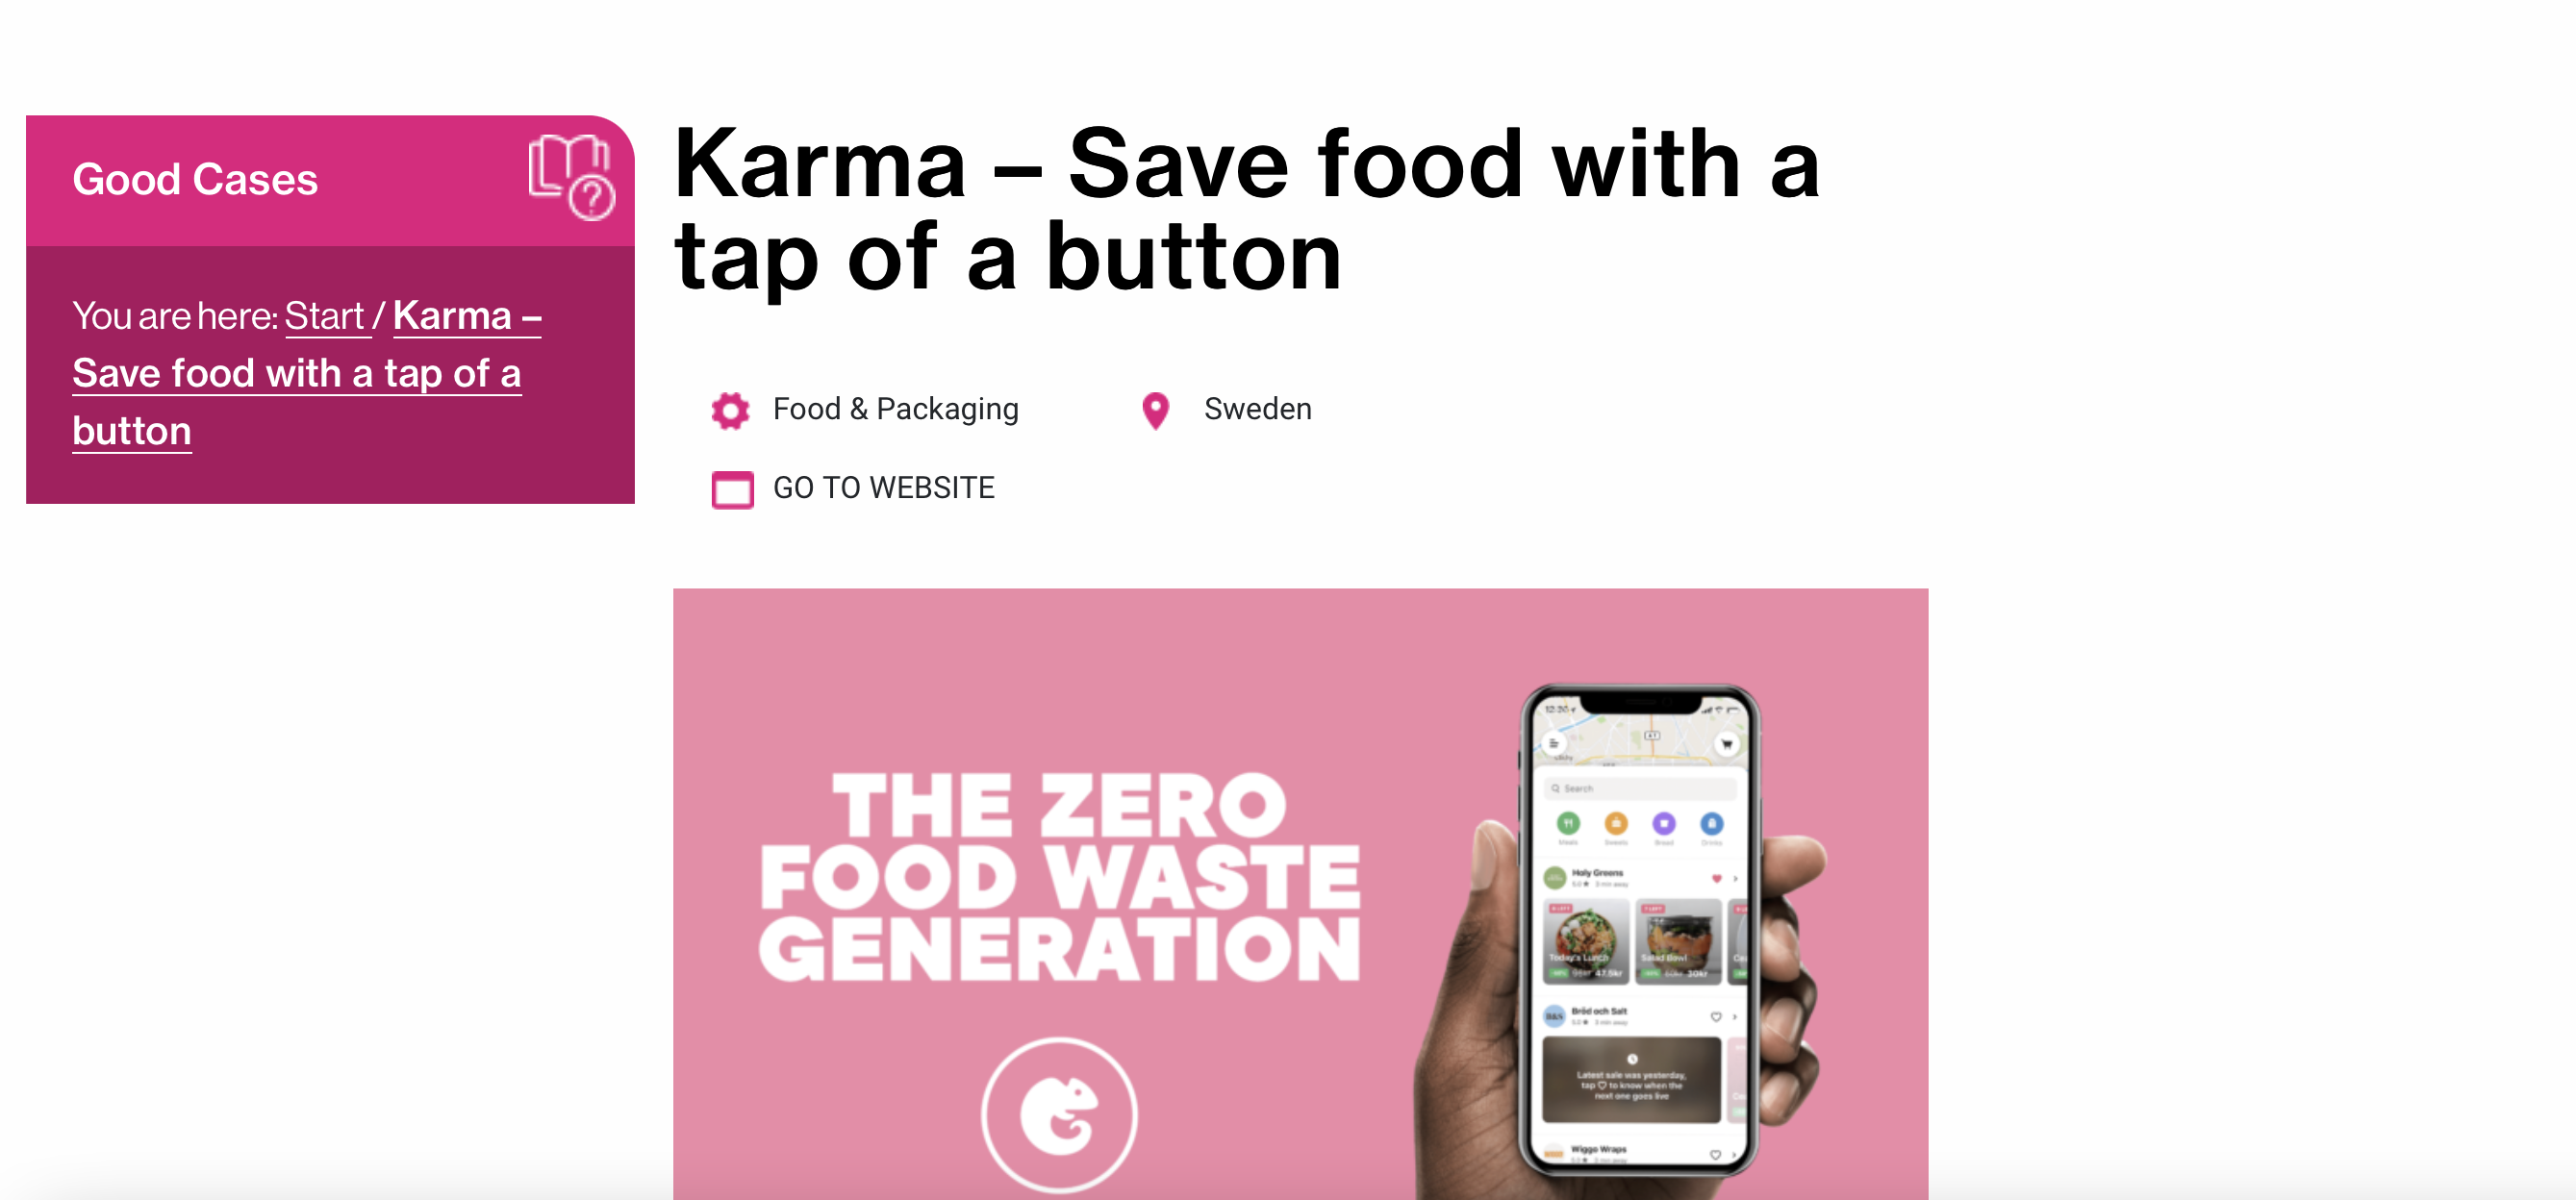
\includegraphics[width=\linewidth,keepaspectratio ]{projectReportTemplate/figures/Karma.png}
    \caption{Karma}
    \label{fig karma}
\end{figure}
\newpage
\subsection{Phenix}
Phenix as shown in Figure \ref{fig pheoinx} is a mobile application. This application helps the users to find the unsold items in nearby store. The products that are not sold for specific time frame will be listed to application so that people near the store can buy these products and help them reduce food waste.\\
\begin{figure}[!h]
    \centering
    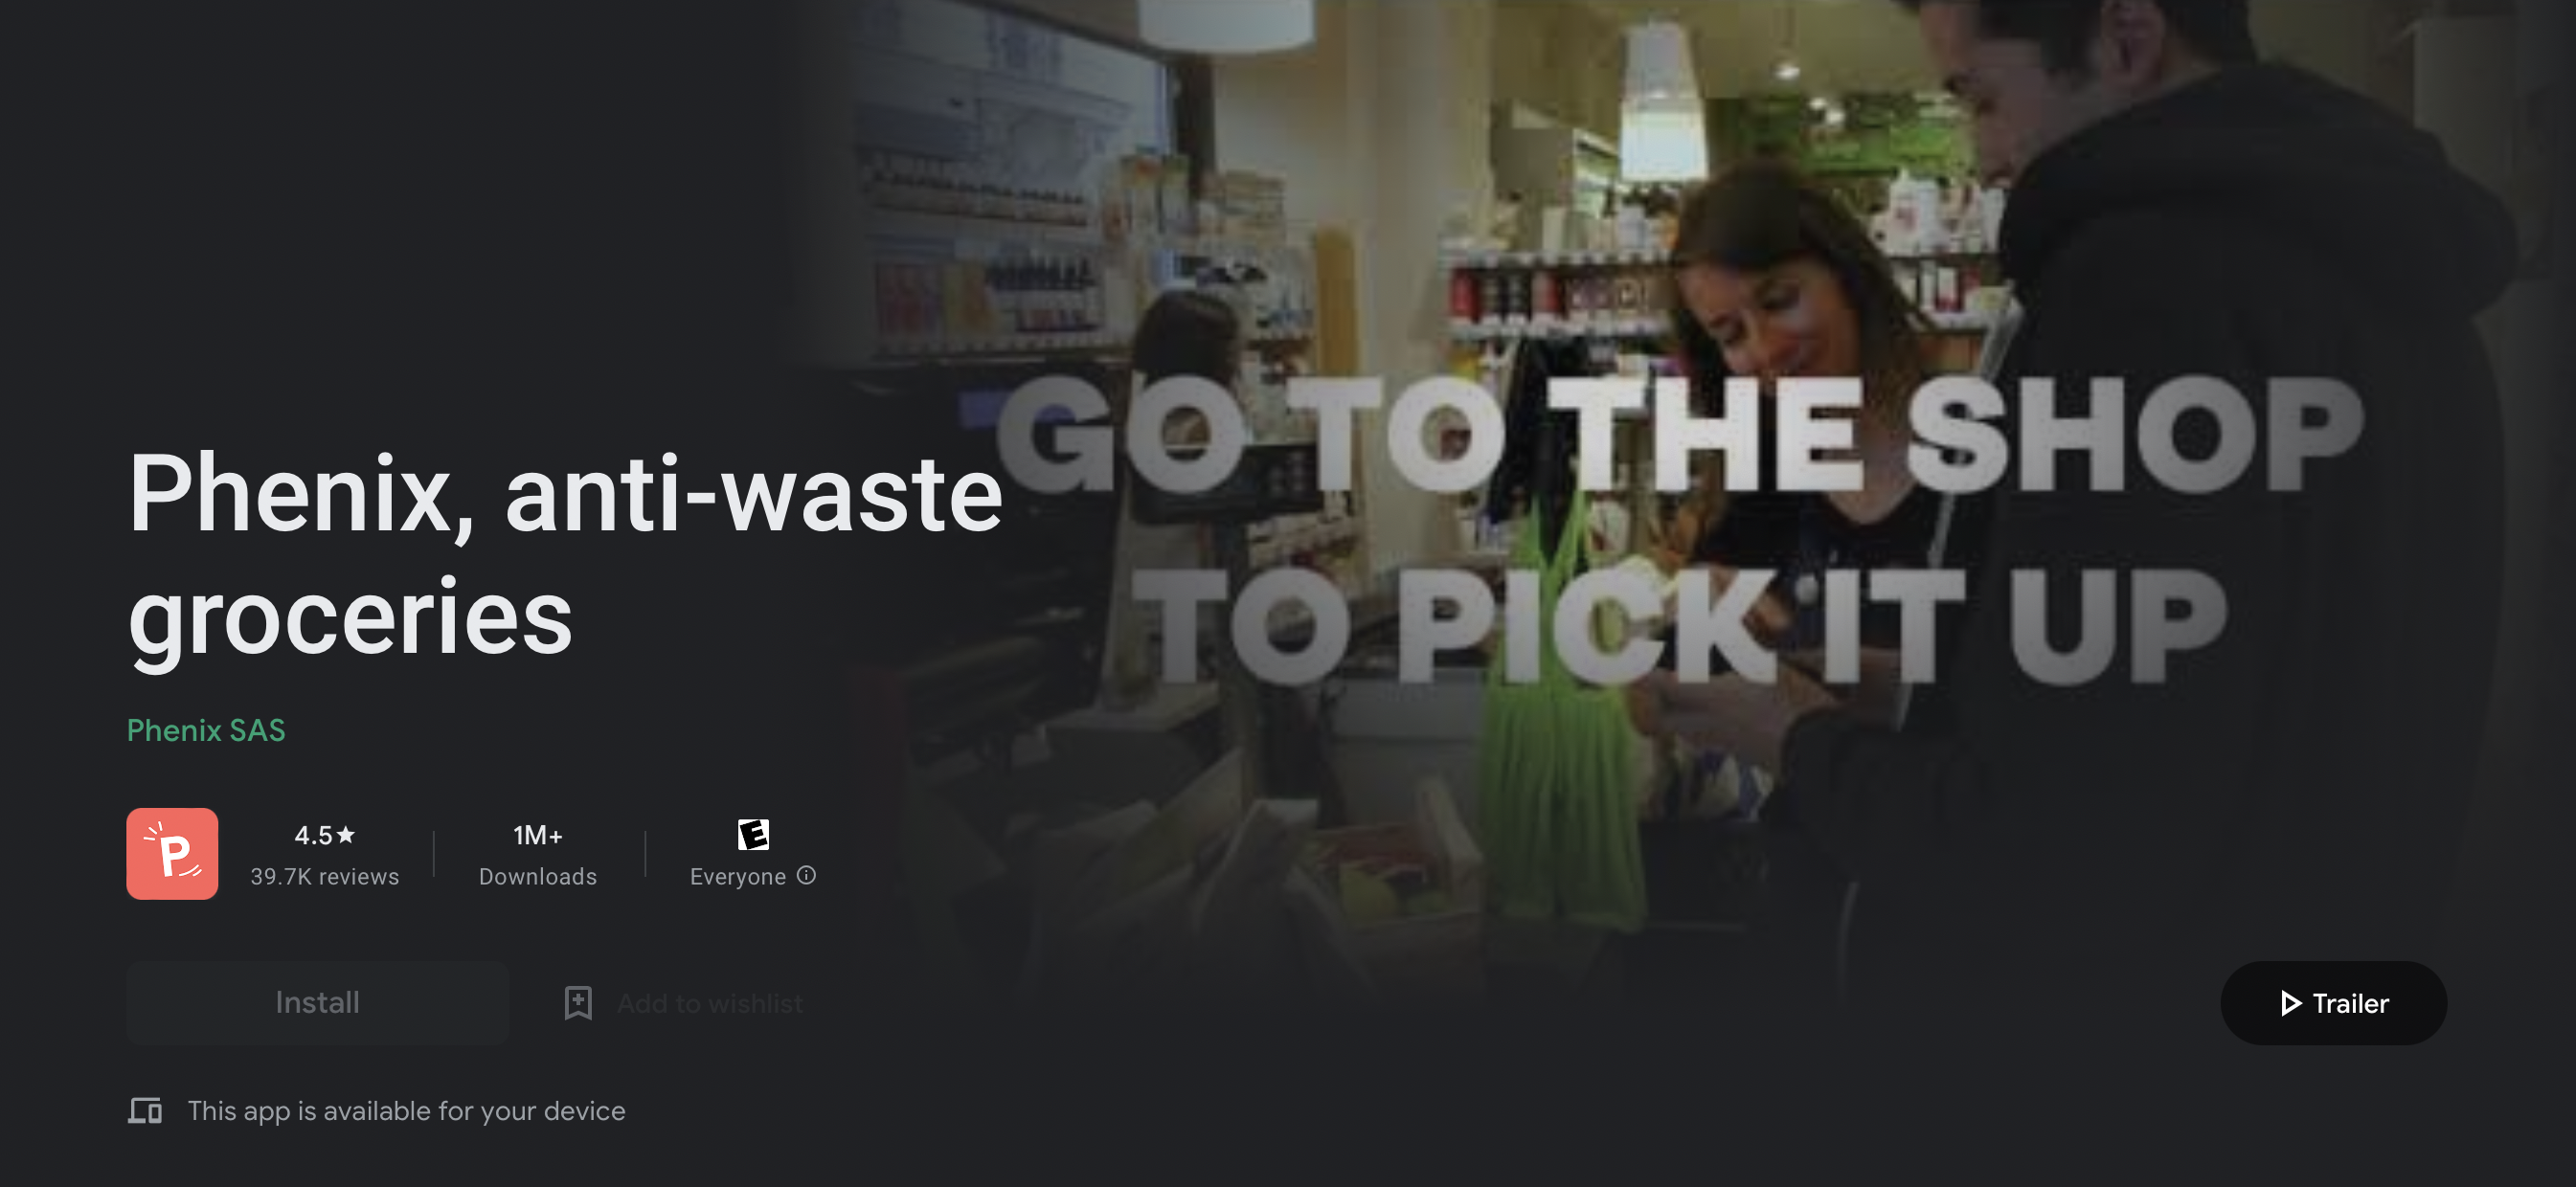
\includegraphics[width=\linewidth,keepaspectratio ]{projectReportTemplate/figures/Phenix.png}
    \caption{Pheonix}
    \label{fig pheoinx}
\end{figure}
\newpage
\subsection{FoodHero}
FoodHero \cite{ref8} as shown in Figure \ref{fig:Foodhero} is mobile appliaction. This application allow users to find food in their local area at lowest price as possilbe. The user simply add the discounted excess food in his cart and then he buys it from store to reduce the excess food wastage.\\
\begin{figure}[!h]
    \centering
    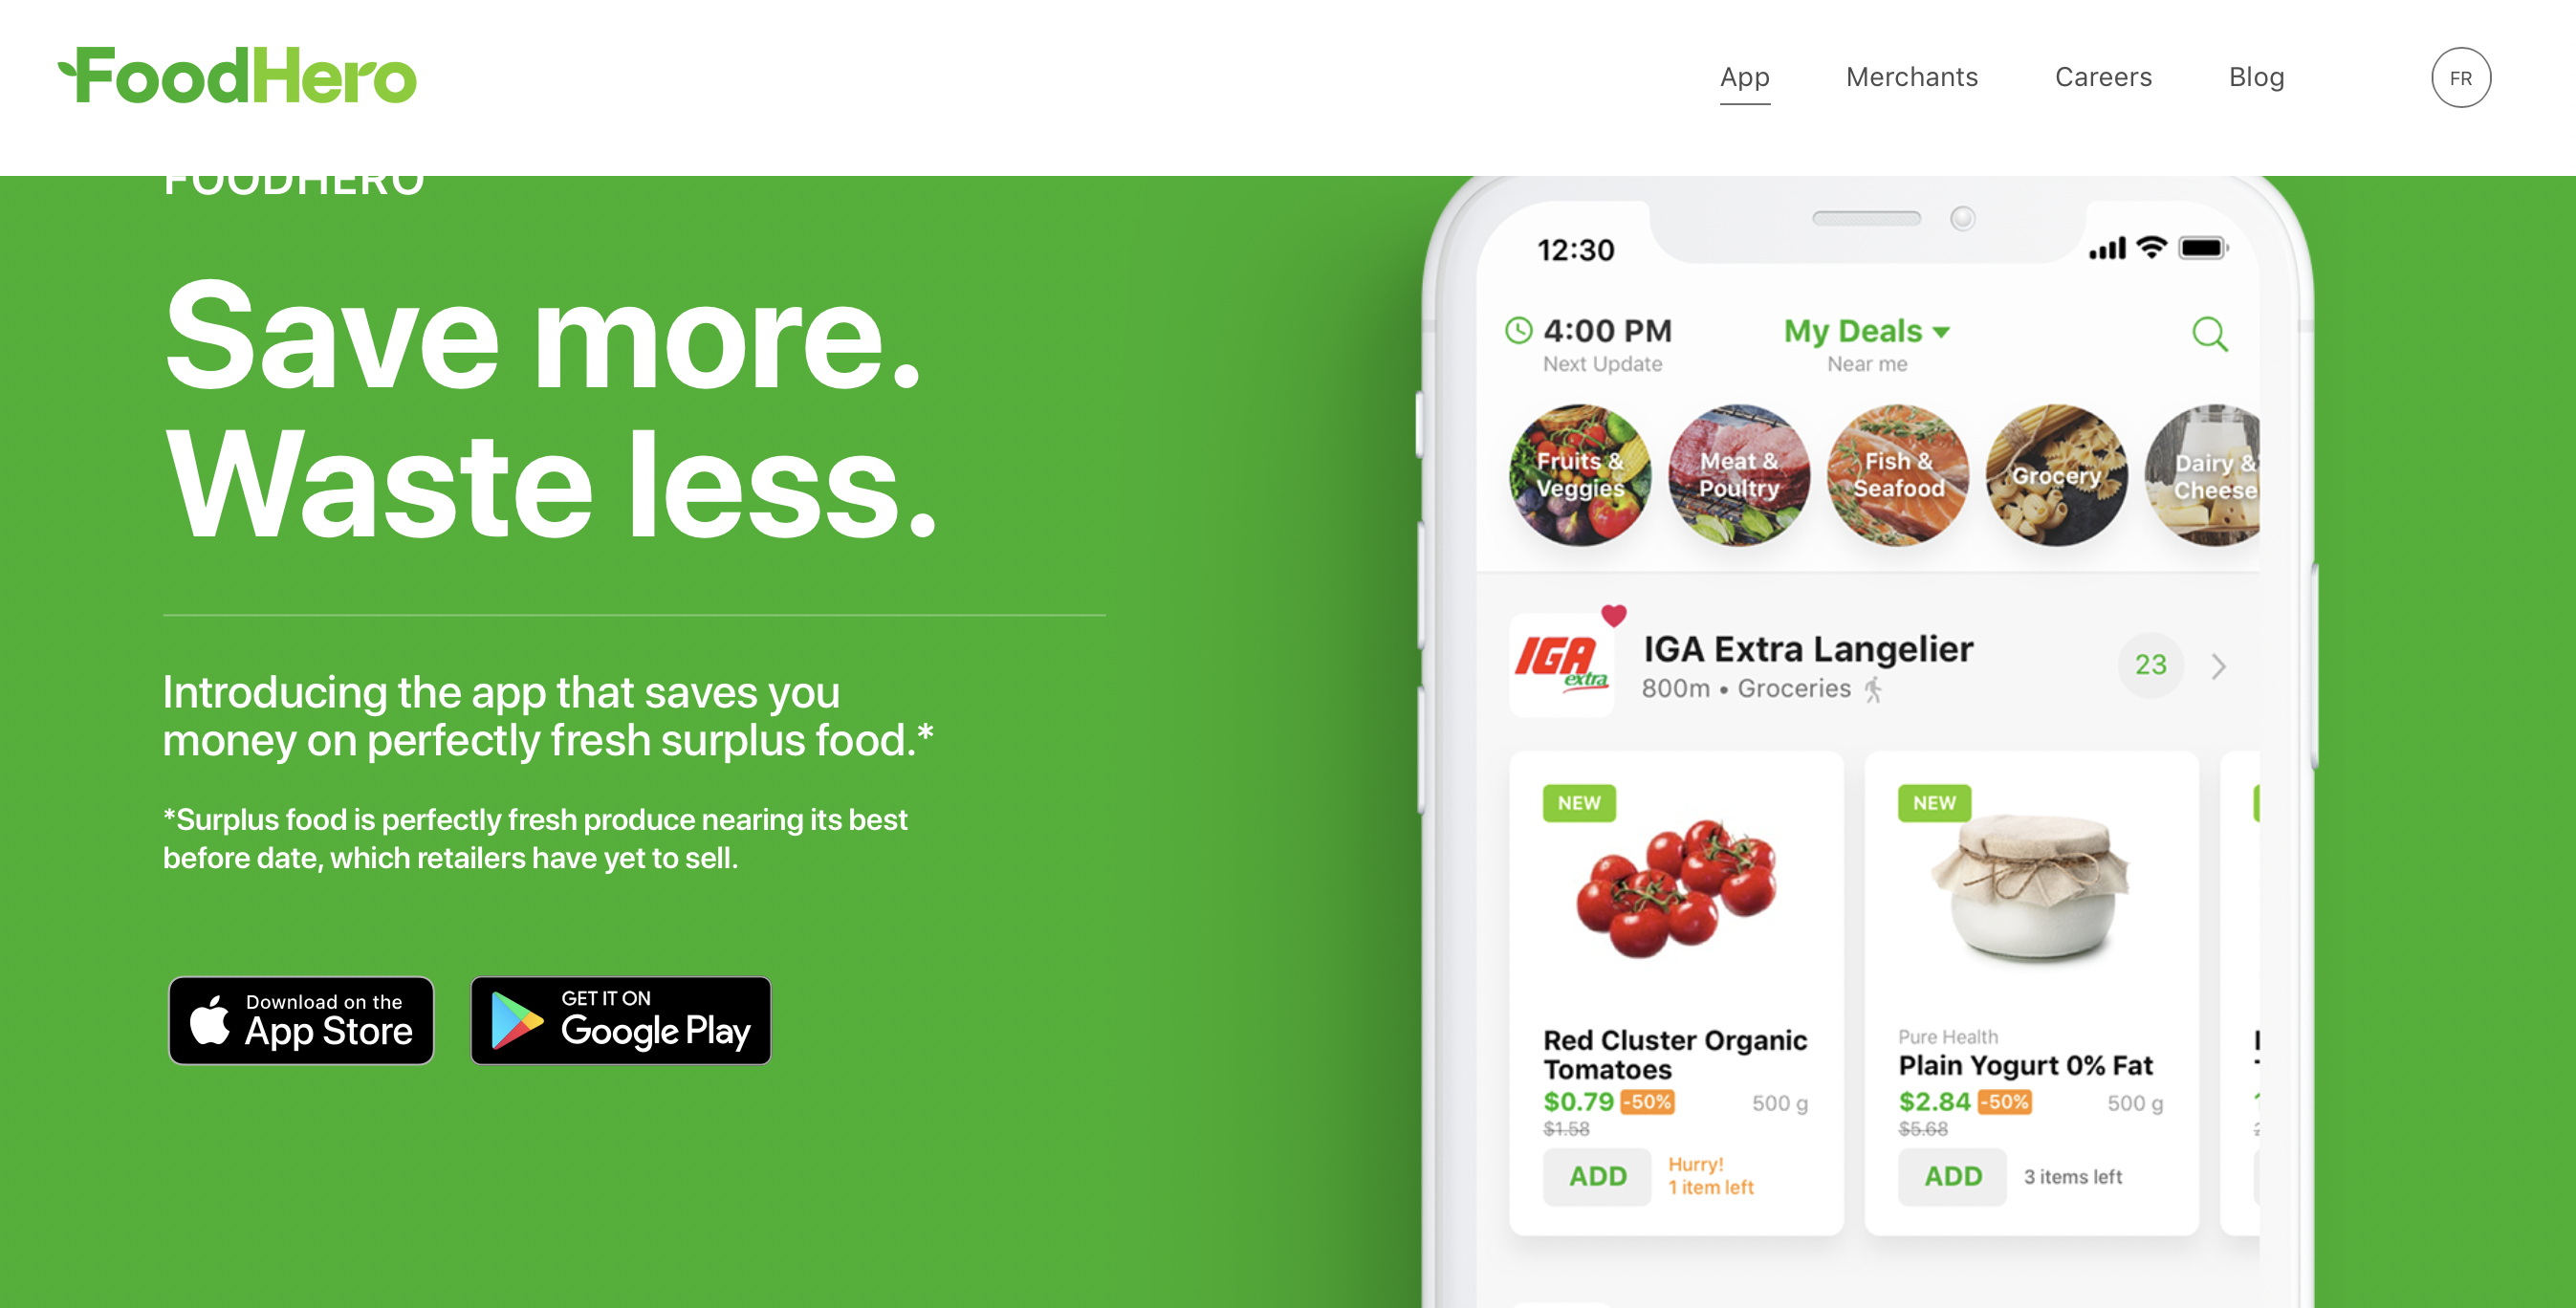
\includegraphics[width=\linewidth, keepaspectratio ]{projectReportTemplate/figures/FoodHero.png}
    \caption{FoodHero }
    \label{fig:Foodhero}
\end{figure}
\newpage
\section{Comparison Table}
The feature Table \ref{tab1} shows the comparison between our web application and our competitor in the same space. The competitor applications shown in the table are mobile base applications. Most of these applications works on free food and donation of food items while, proposed web application works on food bidding. These applications are restricted to mobile users only and the information about the food is only provided when we logged in to the system. Our proposed system provides data transparency and information about food without registration. \\
\begin{table}[!h]
    \centering
    \begin{tabularx}{1\textwidth} { 
  | >{\centering\arraybackslash}X 
  | >{\centering\arraybackslash}X 
  | >{\centering\arraybackslash}X 
  | >{\centering\arraybackslash}X 
  | >{\centering\arraybackslash}X 
  | >{\centering\arraybackslash}X 
  | >{\centering\arraybackslash}X |}
 \hline
 Comparison Table & Too Good To Goo & Olio & Karma & Phenix & Food Hero & Our Web Application\\
 
 \hline
 
 Data Transparency  & $\times$  & $\times$ & $\times$ & $\times$ & $\times$ & \checkmark{} \\

\hline

Bidding System  & $\times$  & $\times$ & $\times$ & $\times$ & $\times$ & \checkmark{}\\

\hline

Use on Mobile  & \checkmark{}  & \checkmark{} & \checkmark{} & \checkmark{} & \checkmark{} & \checkmark{}\\

\hline

Use on Web Browser  & $\times$  & $\times$ & $\times$ & $\times$ & $\times$ & \checkmark{}\\

\hline

\end{tabularx}
    \caption{Feature Table}
    \label{tab1}
\end{table}
 
\doublespacing
\chapter{Requirement Specifications} \label{chap:reqs}

%\version{v1.10.2015}

\section{Requirements}
This chapter include all the functional requirement for the project. It includes system specification, non functional requirements and functional requirements.

\section{Functional Requirements}
The functionality that we use in our web application are listed in the following Table \ref{tab:NonFER} below.


\begin{table}[!h]
    \centering
    \begin{tabular}{|p{3cm}|p{11cm}|}
        \hline 
        Functional requirements & Description of Functional Requirements \\
        \hline
        Register & In this module user will first enter all the requirements of his personal information and then he is going to register in our web application.  \\ 
        \hline
        Login & User that is registered in our application can login in our system. only the logged in  person can bid on our web application on products that are listed on bidding.\\
        \hline
        Profile configuration & In this requirement the user will be able to edit all of his bid related information and also he can change his personal information.\\ 
        \hline
        Forget Password & The user who do not remember his password can simply type is email in forgot password section and he will be sent his password on his email that he registered in our system. \\
        \hline
        Admin & This section will be for the application organizer in which he will manage the application throughout.\\
        \hline
        Bidding & This section will be for bidding of the food products. In this section bidder will add the details of the products and buyer will bid on the product.\\ 
        \hline
        Purchase History & In this section the user will be able to view the purchase history and his bidding.\\
        \hline
        My bidding & User will be able to view his bidding.\\ 
        \hline
        Data Base Search & This section will allow user to bid on desire product and search for it.\\
        \hline
        Contact Us & This section will allow user to send us information via email given in this section.\\
        \hline
        New Bid & In this section user will be able to place his product for the bid and set the price and date for bid. \\
        \hline
        Edit Record & In this section admin and user both will be able to edit the information about the product listed for the bidding.\\
        \hline
        Feedback & In this section the user will be able to give us the information about his experience in our system and can suggest us ways that how we can improve user experience and can also suggest improvements through email.\\
        \hline
        Sales History & In this section the user will be able to see his all previous bids and he can also view previous bids of his clients.\\
        \hline
        Profile Management & In this section the user will be able to edit his profile information and can update his locations based on his products.\\
         \hline
    \end{tabular}
    \caption{Functional Requirements of our application}
    \label{tab:NonFER}
\end{table}
\newpage
\section{Non Functional Requirements}
The Non functional requirements of our web application are following:
\subsection{Availability}
Proposed web application is always available to the user 24/7. All he need is the internet connection to use our web application.
\subsection{Usability}
The usability of web application involve how much friendly the application is to the user. The user can easily learn and user our web application.
\subsection{Reliability}
Proposed web application include no data crash and easy data access when required to the system.
\subsection{Security}
The access between the bidder and seller is always secured and no data is been violated. 
\\

\newpage
\section{System Specifications}
The system specification for our web application are shown in the following Table \ref{tab:System Requirement} below:
\\
\begin{table}[!h]

    \centering
    \begin{tabular}{|p{4cm}|p{10cm}|}
        \hline Software Requirements & Descriptive  \\
        \hline
        VS Code  & The editor we use to built our web application is visual studio code \cite{microsoft_2021}. We use VS Code to built our web application. It is developed by Microsoft and is open source with unlimited features and extensions. It is ranked third for developing applications. \\ 
        \hline
        Angular &Angular is the powerful front end single page application developed by Google and provide a lot of features such components, directives, services, modules, decorators, selectors embedding, routers outlets. It has both eager loading and lazy loading strategies depends upon the developer requirement's. As for as our project is concerned we have implemented both strategies, one for each module and another for sub-components. By default it has eager loading and it also gives us the feature of wild card to move user into page due to entering wrong URL aka 404 page not found.
         \cite{Ang}. \\
        \hline
        MySQL & We are using MySQL \cite{ref3}.The version of MySQL is Version 12.4.3 and SQLYog for editor managing database and all  relations.
        MySQL can Handel, store and modify the information and data about all the actors involve in our system. \\
        \hline
        Node JS & It is 100 times faster and secure than typical PHP. It is non-blocking HTTP request handler which mean that it will not block the next request if there a HTTP request in execution but rather it will be queued and prioritized. It is so powerful that it can handle up to 15000 HTTP per second (RPS) and by using the Vanila HTTP module it can handle up to 700000 requests per minutes.\\
        \hline
    \end{tabular}
    \caption{System Requirements}
    \label{tab:System Requirement}
\end{table}
\doublespacing
\chapter{Design} \label{chap:design}

%\version{v1.10.2015}


\doublespacing
\section{Data Flow Diagram}
The data flow diagram of our application is given below in Figure \ref{fig:DFD}. It explains that we have three components and each component interact with each other by sending request while doing their task fulfill.
\begin{figure}[!h]
    \centering
    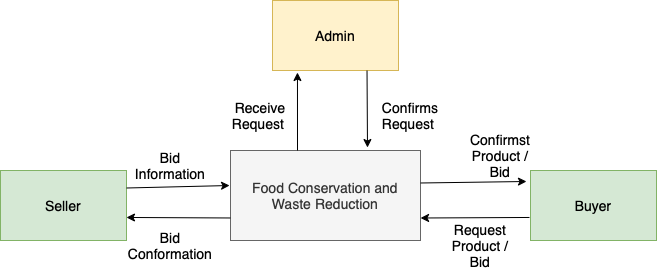
\includegraphics[width=15cm, height=15cm, keepaspectratio ]{Data Flow Diagram.drawio-2.png}
    \caption{Data Flow Diagram}
    
    \label{fig:DFD}
\end{figure}
\newpage
\section{Sequence Diagram}
This is the sequence diagram of our web application and it is the  representation of the system as whole, how buyer and seller will login to our system. The Buyer is going to create a bid. The request will transfer to the bid manager then it is going to come back with result. Same will happen to Bidding, The bid manager sends the request to bidding and then bidding will update the status of the product that is on bid. The sequence diagram of our web application is listed below in Figure \ref{fig:SD} : \\
\begin{figure}[!h]
    \centering
    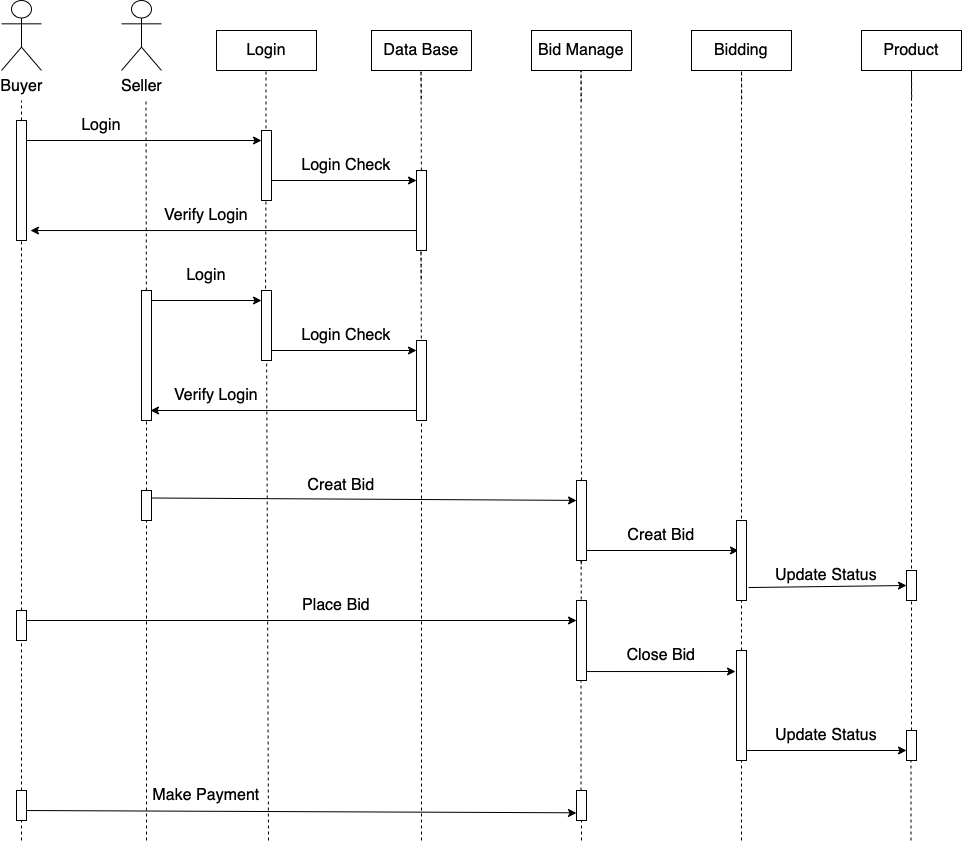
\includegraphics[width=15cm, height=15cm, keepaspectratio ]{Updated Final Sequence Diagram.drawio.png}
    \caption{Sequence Diagram of system}
    \label{fig:SD}
\end{figure}
\section{Use Case Diagram}
The use case diagram of our web application explains how user is going to interact in our application. The all the functionalities that user can perform in our web application is represented in usecase figure \ref{fig:UCD1}, \ref{fig:UCD2}. The users for our web application will be buyer, seller and admin and their use cases are following.

\subsection{For Users}
The use case diagram for Buyers and Sellers is shown in following Figure \ref{fig:UCD1}. The buyer can sign up and sign in to the system. Buyer can search for the product, apply for bid and browse items in the system. The seller can sign up and sign in to the system. Seller can manage item, place items for bidding. \\
\begin{figure}[!h]
    \centering
    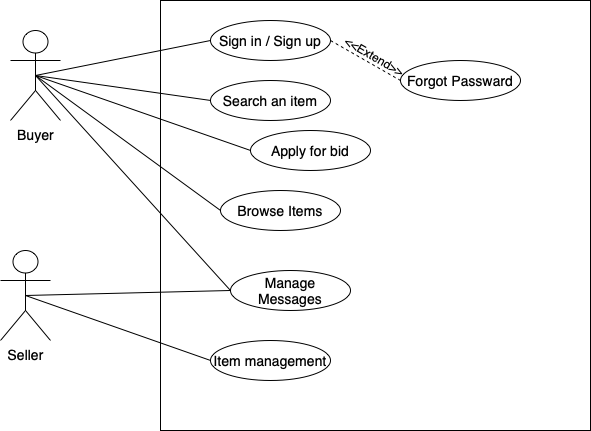
\includegraphics[width=15cm, height=15cm, keepaspectratio ]{Usecase Diagram Diagram.drawio.png}
    \caption{Use Case Diagram For Users}
    \label{fig:UCD1}
\end{figure}
\newpage
\subsection{For Admin}
The use case diagram for Admin is shown in following Figure   \ref{fig:UCD2}. The admin can login to the system. Admin can manage items like modify data about items, access data of items. Admin can manage users in the system.\\
\begin{figure}[!h]
    \centering
    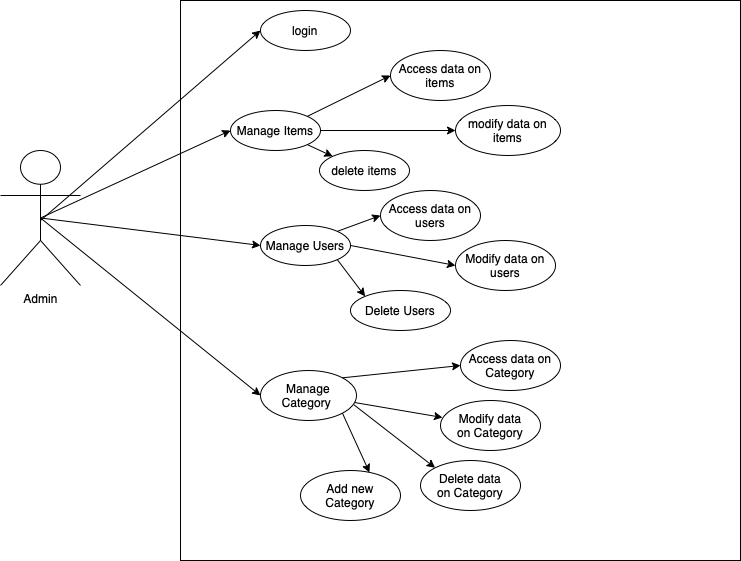
\includegraphics[width=15cm, height=15cm, keepaspectratio ]{Usecase Admin.drawio.png}
    \caption{Use Case Diagram For Admin}
    \label{fig:UCD2}
\end{figure}

\section{Activity Diagram}
The activity diagram of our web application representation all the activities throughout our web application. In these diagrams you will be able to see clear overview of our web application.

\subsection{For Sign Up/Login In}
The activity diagram for Sign up and Login is in following Figure \ref{fig:AD1}. The users enters the login page. If user is registered then user will be simply logged in. The new user will register first and then enters in the web application to perform bidding. \\
\begin{figure}[!h]
    \centering
    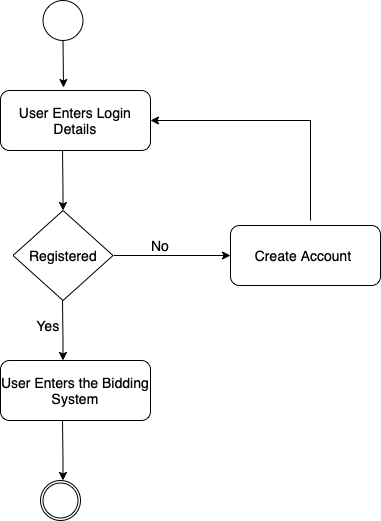
\includegraphics[width=15cm, height=15cm, keepaspectratio ]{Activity Diagram.drawio.png}
    \caption{Activity Diagram For Sign Up/Login}
    \label{fig:AD1}
\end{figure}

\subsection{For Bidding}
The activity diagram for complete process of bidding is shown in following Figure \ref{fig:AD2}. The user will first search for the item. If the item is available then user will check if the bidding is open on the searched item. The user will then apply bid on the item. If user won the bid, user will be notified. Then user will proceed to the payment method.
\begin{figure}[!h]
    \centering
    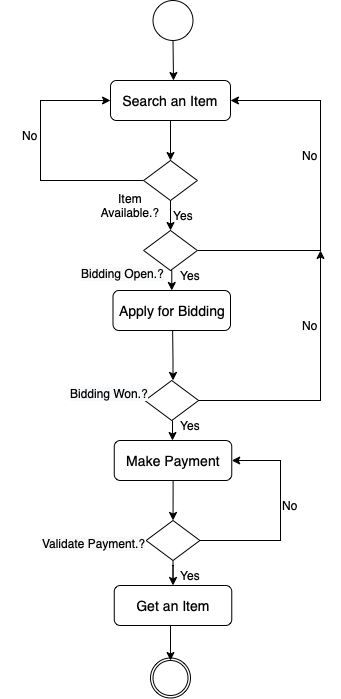
\includegraphics[width=15cm, height=15cm, keepaspectratio ]{Activity Diagram Process.drawio.png}
    \caption{Activity Diagram For Bidding}
    \label{fig:AD2}
\end{figure}
\newpage
\section{ER Diagram}
\doublespacing
\textbf{Entities}
 \\
\textbf{User:} This entity captures information about the buyer or seller who signed up on our web application portal.\\
\textbf{Administrator:} The entity captures the information about all the individuals who are responsible for the functioning of web application.\\
\textbf{Product:} This entity captures the information about all the products which are available for the Bidding.\\
\textbf{Bidding:} This entity captures the information about any product which is already on a bid.\\
\textbf {Feedback:} This entity captures the information about reaction/feedback of any buyer or seller about any product on bidding.\\
\textbf{Bid:} This entity captures the information about the bid any buyer has put for a product i.e. the price a buyer is willing to pay in an bidding.\\
\textbf{Payment Method:} This entity captures the information about chosen payment method for any sold product by a buyer or accepted payment methods by seller for any product.
The following is ER Diagram shown in Figure \ref{fig:ER} :\\
\begin{figure}[!h]
    \centering
    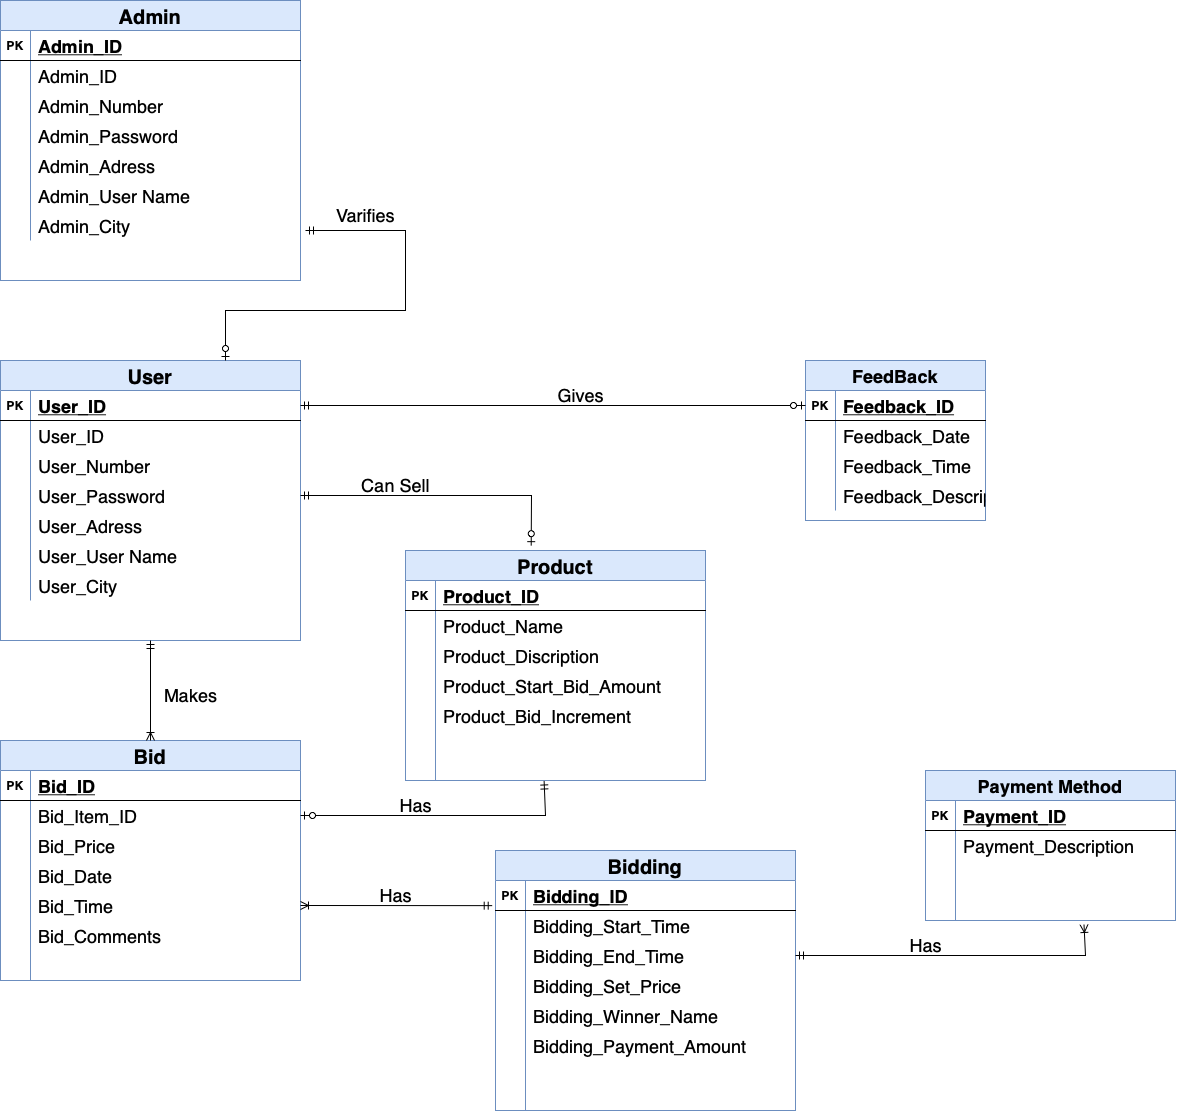
\includegraphics[width=15cm, height=15cm, keepaspectratio ]{Final ER Diagram.drawio.png}
    \caption{ER Diagram}
    \label{fig:ER}
\end{figure}\\
\newpage
\section{Deployment Diagram}
The Deployment Diagram of our web application is shown in following Figure \ref{DD}. The deployment diagram shows the relation between hardware and software in the system and the processing distribution. The components of the web application runs on across the devices shows physical arrangement of nodes in distributed system.  \\\\

\begin{figure}[!h]
    \centering
    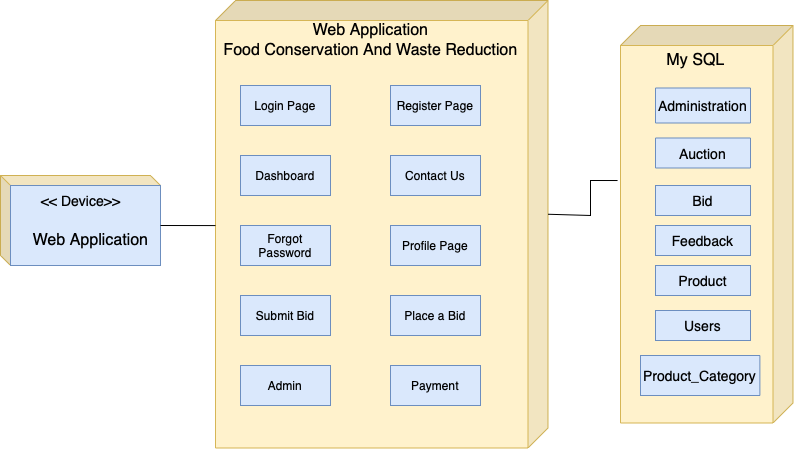
\includegraphics[width=15cm, height=15cm, keepaspectratio ]{projectReportTemplate/figures/Deployment Diagram.drawio.png}
    \caption{Deployment Diagram}
    \label{DD}
\end{figure}
\newpage
\section{Component Diagram}
The Component Diagram of our web application is shown in following Figure \ref{CD}. The component diagram helps in wiring the physical components in the system. The bidding, payment, contact us, managing users are all carried out thought the data base. and all of these are either done by users of the web application or admin.\\\\

\begin{figure}[!h]
    \centering
    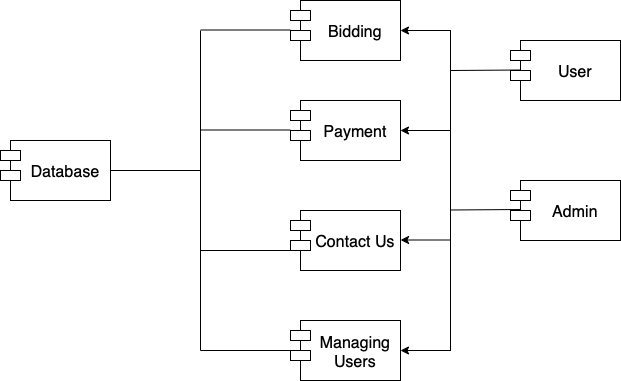
\includegraphics[width=15cm, height=15cm, keepaspectratio ]{projectReportTemplate/figures/Component Diagram.drawio.png}
    \caption{Component Diagram}
    \label{CD}
\end{figure}

\doublespacing
\chapter{System Implementation} \label{chap:sysImplementation}
%\version{v1.10.2015}

\doublespacing

The software and hardware requirement that was required to built our web application are following:\\
\section{Hardware Requirements}
Following are the hardware requirements of the proposed system:\\
•	Processors : Quad core system.\\
•	RAM : Minimum ram is 4GB.\\
•	HDD : At least 20GB.
\section{Software Requirements}
Following are the software requirements of the proposed system:
•	MS VSCode or MyEclipse : For front-end and back-end developments.\\
•	Postman : For testing the API’s before checking it by using HTTP requests.\\
•	SQL YOG : For database management.\\  
•	Browsers/clients like chrome for testing the output of the system design.
\newpage
\section{UI Implementation}
\subsection{Home Page}
When user visit in our web application he will enter to home page. The home page of our web application is shown in following Figure \ref{HPl}.All the information about bidding will be shown in home page. He can place bid only if he is login in our web application. In case of invalid URL in search. The Visitors  will be moved to 404 not found page which angular provide as wild card in routing and navigation listed at the last of routing.\\
\begin{figure}[h]
    \centering
    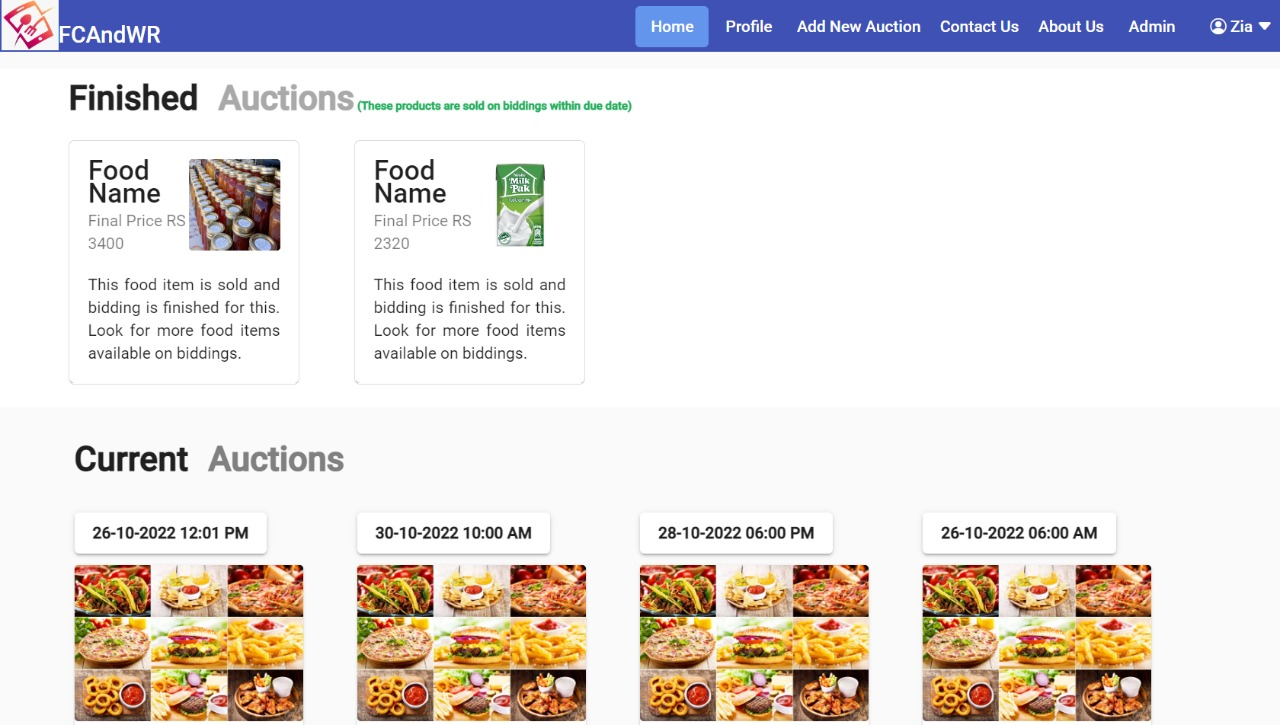
\includegraphics[width=15cm, height=15cm, keepaspectratio]{Homepage.jpeg}
    \caption{Home Page}
    \label{HPl}
\end{figure}

\subsection{Profile Page}
This page shows the user purchase history and user sales history. when a user won a bid he will be able to see his won bid in his profile section. The profile page of our web application is shown in following Figure \ref{pp}.
\begin{figure}[!h]
    \centering
    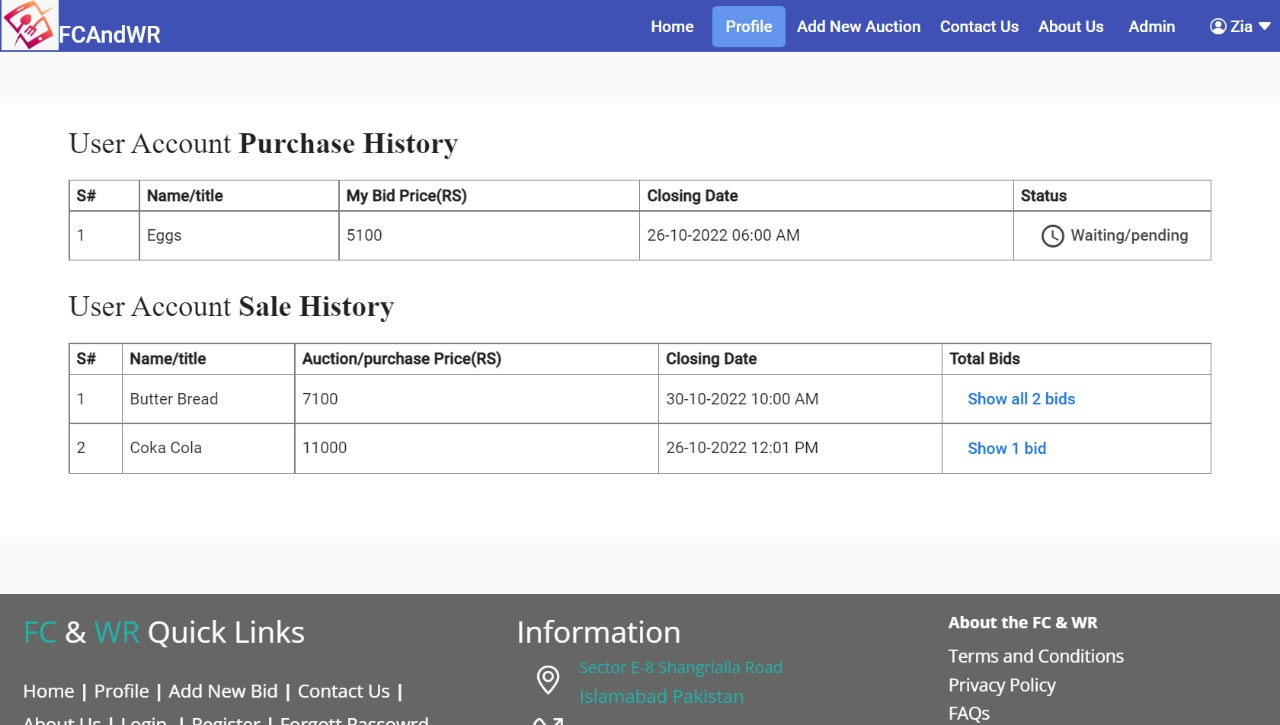
\includegraphics[width=15cm, height=15cm, keepaspectratio]{profile.jpeg}
    \caption{Profile Page}
    \label{pp}
\end{figure}

\doublespacing
\chapter{System Testing And Evaluation}\label{chap:testingEvaluation}

%\version{v1.11.2015}

\section{Evaluation And Testing of the System }
\doublespacing
This phase includes testing every interface functionality of the website application. This will help us in executing the results against our requirements specified by going through different scenarios. All of the modules will be tested to know their working and functionalities properly. For this purpose, the modules in our web which are Home, Login, User Account Configuration, Profile, Admin, Contact Us, About Us, and Add New Auctions are tested properly an working as expected.
\section{Testing Of System GUI}
\doublespacing
All parts of the web which are used by site visitors, and visible parts of the site to interact with our web application are tested in this stage of system evaluation. For this purpose, we have implemented interfaces that are easy to understand, with a proper feedback and user engagement techniques. The interfaces are structured in a self-explanatory way. An example is the new user registration interface. If someone visits and just looks for a minute can easily understand the interface. The feedback that we have provided like success messages, error prompts, loaders, buttons,s and sections clicking ripples will know the user position and system status. Other helping materials like icons provided by Bootstrap, Google, and Angular material Io are specialized for user help throughout the process of interacting with the interface.
\section{Integration Testing Of Web Application}
\doublespacing
This stage of system evaluation is the overall testing of modules included in the application in the group in a proper sequence. We have to make sure that there are no errors occurring throughout the integration testing and safe navigation as well as invoking/initializing/instantiating of new modules. For this purpose, we have tested our website by registration of the new user, creating new auctions, listing the home current auction section to buyers aka bidders, list of all bids against an auction, and informing the seller and bidder. On confirming/approving a bid, the bidder is informed and asked to checkout. Once the bidder/buyer pays for the auction the seller is informed and the auction is moved from status In bidding to Sold and the section is changed to finished auctions.Integration testing further explained below:
\subsection{For Login}
\doublespacing
To place a bid or create their own auction the visitor has to log in themselves. The interface will ask them for the user's email address and password. By submitting the user will be verified from the database. On valid details, the user will be navigated to Home Page and in case of invalid details, the user will be informed with error alerts and will not be navigated to any other Page.ck whether he is an authentic logged in user.
\subsection{Registration Of New Entrants}
\doublespacing
This interface is for fresh site visitors. Visitors have to provide all the mandatory fields marked with the * sign and other validators. Each and every input field has its own validator like the name not being null, a minimum length of 3, and a maximum of 30 characters. Password is mandatory, min length of 4 and a maximum of 12 characters. On valid details, all the errors will be hidden and the form status is VALID. On submitting a loader will show for saving into the database and provide feedback to users.
\section{Compatibility Testing}
\doublespacing
Compatibility means the application is working across different platforms. Our project is a web-based application that should be compatible with all browsers. Our web application is compatible with renowned browsers like Google Chrome, Safari, Mozilla Firefox, MS Edge. The language for the development of the front end is Angular which is developed by Google and is undoubtedly compatible across all browsers.

\section{Usability Testing}
\doublespacing
This phase of testing the web application is to involve users checking whether it is easy to use or not, easy to learn, or whether users face difficulties. This test is conducted through the following factors:
\subsection{Easy To Use}
To judge the application level easiness for users. For this purpose we have used animations, icons, signatures, notifications, and loaders to keep users engaged.
\subsection{Safe To Use}
Unintended actions by users will not destroy their whole efforts. An example will help us. Suppose a user is registering and mistakenly click clear all fields instead of submitting the form, the application will ask for user confirmation. After the user confirm his/her actions decisions are made. 
\subsection{Engaging And Pleasing Users Experience}
Looks matters. Icons like satisfied emojis, success colors, animations, and the nice look of the interface. All these kinds of stuff will engage and please the user and will use it again and again.
\subsection{Application Is Memorable}
Once the user uses the app and revisits it after some time. Users can leave, or return whenever they urge to use the application. Our interfaces are designed in a way that it will remember the users if they revisit after some time.
\newpage
\section{Unit Testing}
\doublespacing
In our web application, we test every module individually. The module we have tested are below.
\subsection{Registration Test Successful}
Registration Test Case Positive is shown in Figure \ref{tt1}.
\begin{table}[!h]
    \centering
    \begin{tabular}{|p{5cm}|p{8cm}|}
        \hline
        \textbf{Test ID} & \textbf{TI-1}\\
        \hline
        \textbf{Tested Function} &  Successfully user registers. \\
        \hline
        \textbf{Initial State of application} & All fields are empty.\\
        \hline
        \textbf{Input} & User enter the valid data.\\
        \hline
        \textbf{Expected Output} &  Successfully registered in system.\\
        \hline
        \textbf{Actual Output} & Successfully registered in system.\\
         \hline
         \textbf{Status of the system} & Passed.\\
         \hline
    \end{tabular}
    \caption{Registration Test Successful }
    \label{tt1}
\end{table}
\subsection{Registration Test Unsuccessful}
Registration Test Case Negative is shown in Figure \ref{tt2}.
\begin{table}[!h]
    \centering
    \begin{tabular}{|p{5cm}|p{8cm}|}
        \hline
        \textbf{Test ID} & \textbf{TI-2}\\
        \hline
        \textbf{Tested Function} & Unsuccessfully user registrars. \\
        \hline
        \textbf{Initial State of application} & All fields are empty.\\
        \hline
        \textbf{Input} & User did not enter the valid data.\\
        \hline
        \textbf{Expected Output} & Unsuccessfully registered.\\
        \hline
        \textbf{Actual Output} & Unsuccessful registered.\\
         \hline
         \textbf{Status of the system} & Failed.\\
         \hline
    \end{tabular}
    \caption{Registration Test Unsuccessful}
    \label{tt2}
\end{table}
\newpage
\subsection{Login Test Successful}
Login Test Case Positive is shown in Figure \ref{tt3}.
\begin{table}[!h]
    \centering
    \begin{tabular}{|p{5cm}|p{8cm}|}
        \hline
        \textbf{Test ID} & \textbf{TI-3}\\
        \hline
        \textbf{Tested Function} &  Successful user login. \\
        \hline
        \textbf{Initial State of application} & All fields are empty.\\
        \hline
        \textbf{Input} & User enter valid data.\\
        \hline
        \textbf{Expected Output} &  Successful login.\\
        \hline
        \textbf{Actual Output} & Successful login.\\
         \hline
         \textbf{Status of the system} & Passed.\\
         \hline
    \end{tabular}
    \caption{Login Test Successful}
    \label{tt3}
\end{table}
\subsection{Login Test Unsuccessful}
Login Test Case Positive is shown in Figure \ref{tt4}.
\begin{table}[!h]
    \centering
    \begin{tabular}{|p{5cm}|p{8cm}|}
         \textbf{Test ID} & \textbf{TI-4}\\
        \hline
        \textbf{Tested Function} & Unsuccessful user Login. \\
        \hline
        \textbf{Initial State of application} & All fields are empty.\\
        \hline
        \textbf{Input} & User did not enter the valid data.\\
        \hline
        \textbf{Expected Output} & Unsuccessful Login.\\
        \hline
        \textbf{Actual Output} & Unsuccessful Login\\
        \hline
         \textbf{Status of the system} & Failed.\\
         \hline
    \end{tabular}
    \caption{Login Test Unsuccessful}
    \label{tt4}
\end{table}
\newpage
\subsection{Bid Test Successful}
Bid Test Case Positive is shown in Figure \ref{tt5}.
\begin{table}[!h]
    \centering
    \begin{tabular}{|p{5cm}|p{8cm}|}
        \hline
        \textbf{Test ID} & \textbf{TI-5}\\
        \hline
        \textbf{Function To Be Tested} & Successfully place bid. \\
        \hline
        \textbf{Initial State} & Bid page.\\
        \hline
        \textbf{Input} & Enter all valid bid data.\\
        \hline
        \textbf{Expected Output} & Bid should be placed.\\
        \hline
        \textbf{Actual Output} & Bid is placed.\\
         \hline
         \textbf{Status of the system} & Pass.\\
         \hline
    \end{tabular}
    \caption{Bid Test Successful}
    \label{tt5}
\end{table}

\subsection{Bid Test Unsuccessful}
Bid Test Case Negative is shown in Figure \ref{tt6}.
\begin{table}[!h]
    \centering
    \begin{tabular}{|p{5cm}|p{8cm}|}
        \hline
        \textbf{Test ID} & \textbf{TI-6}\\
        \hline
        \textbf{Function To Be Tested} & Place Bid successful. \\
        \hline
        \textbf{Initial State} & Bid page.\\
        \hline
        \textbf{Input} & Enter invalid bid data.\\
        \hline
        \textbf{Expected Output} & Bid should not be placed.\\
        \hline
        \textbf{Actual Output} & Bid is not placed.\\
         \hline
         \textbf{Status of the system} & Fail.\\
         \hline
    \end{tabular}
    \caption{Bid Test Unsuccessful}
    \label{tt6}
\end{table}
\doublespacing
\chapter{Conclusions}\label{chap:conclusions}
%\version{v1.10.2015}
The conclusion of our final year project is describe below.
\section{Project Conclusion}
Food conservation and waste reduction is a web application in which a company or organization having products near to the expire date or any hotels or marquees having excess food can simply register in our web application and then they upload details about the product, set the price of bid and place end time for the bid. The seller will be shown top bids and the one with the highest bid will win the product and user will be sent to payment page for further processing and finally user can pick the product from given location.
\section{Limitations}
\textbf{1} : Internet connection is always required to access the data from our website.\\
\textbf{2} : The slow speed of loading of online picture contents when retrieved from data base.\\
\textbf{3} : Security risk posed by threat vectors.

\section{User Guide}
The user guide contains step by step process of using our web application form registration in web application to buy the product in the system.\\
\subsection{Home Page}
When user visit in our web application he will enter to home page. The home page of our web application is shown in following Figure \ref{HPl}.All the information about bidding will be shown in home page. He can place bid only if he is login in our web application. In case of invalid URL in search. The Visitors  will be moved to 404 not found page which angular provide as wild card in routing and navigation listed at the last of routing.\\
\begin{figure}[h]
    \centering
    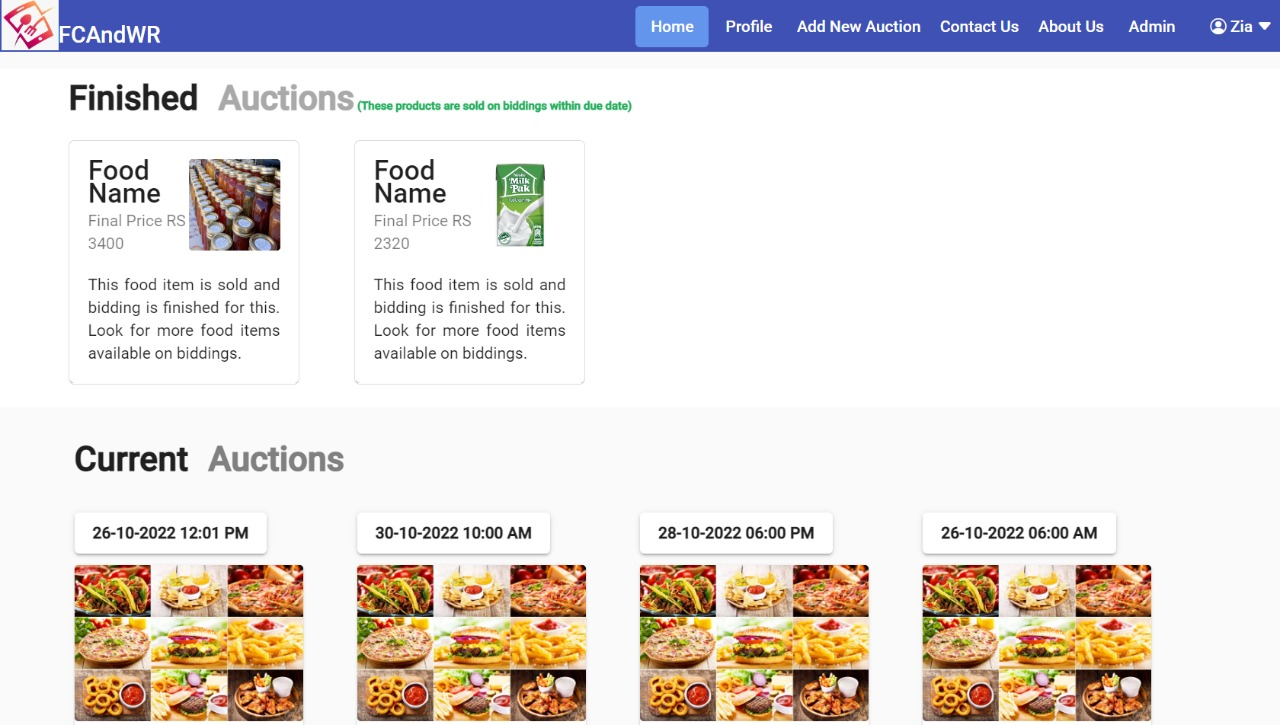
\includegraphics[width=15cm, height=15cm, keepaspectratio]{Homepage.jpeg}
    \caption{Home Page}
    \label{HPl}
\end{figure}
\subsection{Login Page}
After successfully getting register into our web application, user simply need to enter his email and password for login. The login page of our web application is shown in following Figure \ref{lp}.\\
\begin{figure}[!h]
    \centering
    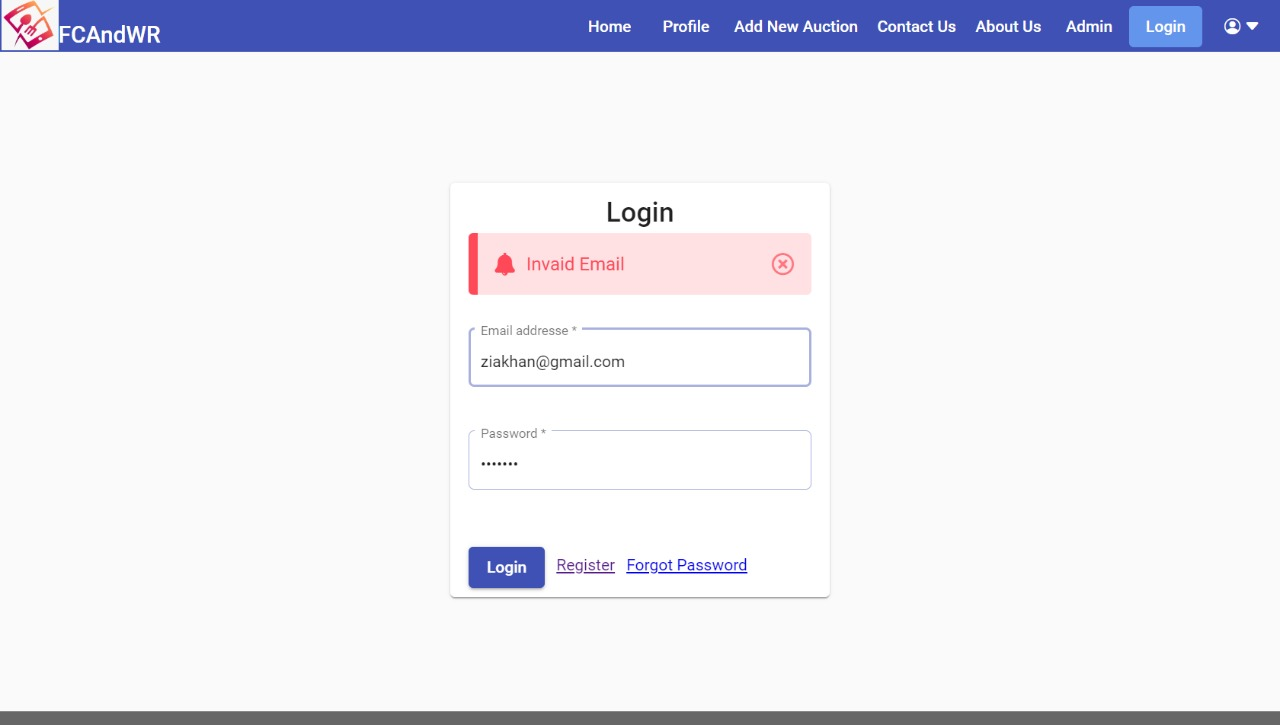
\includegraphics[width=15cm, height=15cm, keepaspectratio]{login page.jpeg}
    \caption{Login Page}
    \label{lp}
\end{figure}
\newpage
\subsection{Login Page Requirements}
If user will Press the login button, then an error will be thrown to him to notify that he must fill all the required credentials. The login page with required field of our web application is shown in following Figure \ref{Lrf}.
\begin{figure}[!h]
    \centering
    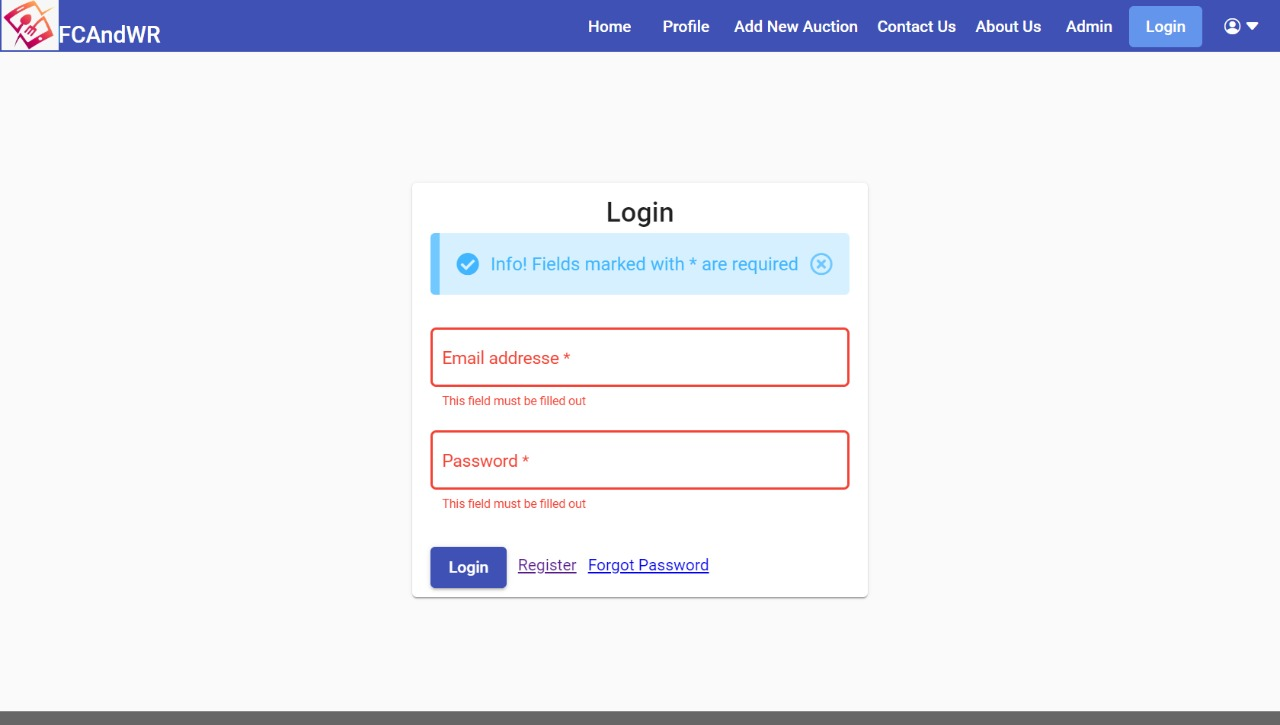
\includegraphics[width=15cm, height=15cm, keepaspectratio]{Login required.jpeg}
    \caption{Responsive Login Page}
    \label{Lrf}
\end{figure}


\subsection{Registration Page}
If the user wants to perform bidding or take part in it, he will first register in application by entering his name, phone number, email address, city, and his address. The registration page of our web application is shown in following Figure \ref{rp}.\\
\begin{figure}[!h]
    \centering
    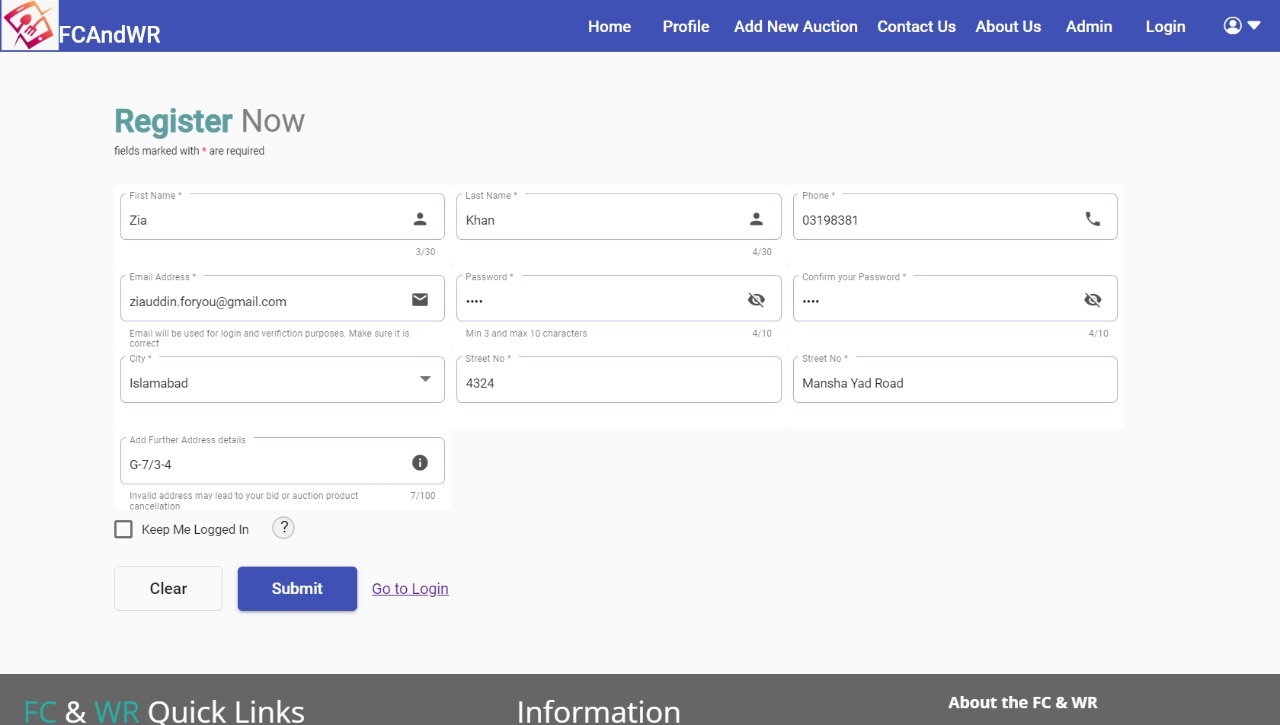
\includegraphics[width=15cm, height=15cm, keepaspectratio]{Register Page.jpeg}
    \caption{Register Page}
    \label{rp}
\end{figure}

\subsection{Registration Page Requirements}
If user will press the login button, then an error will be thrown to him to notify that he must fill all the required credentials. The registration page with requirements of our web application is shown in following Figure \ref{rpr}.
\begin{figure}[!h]
    \centering
    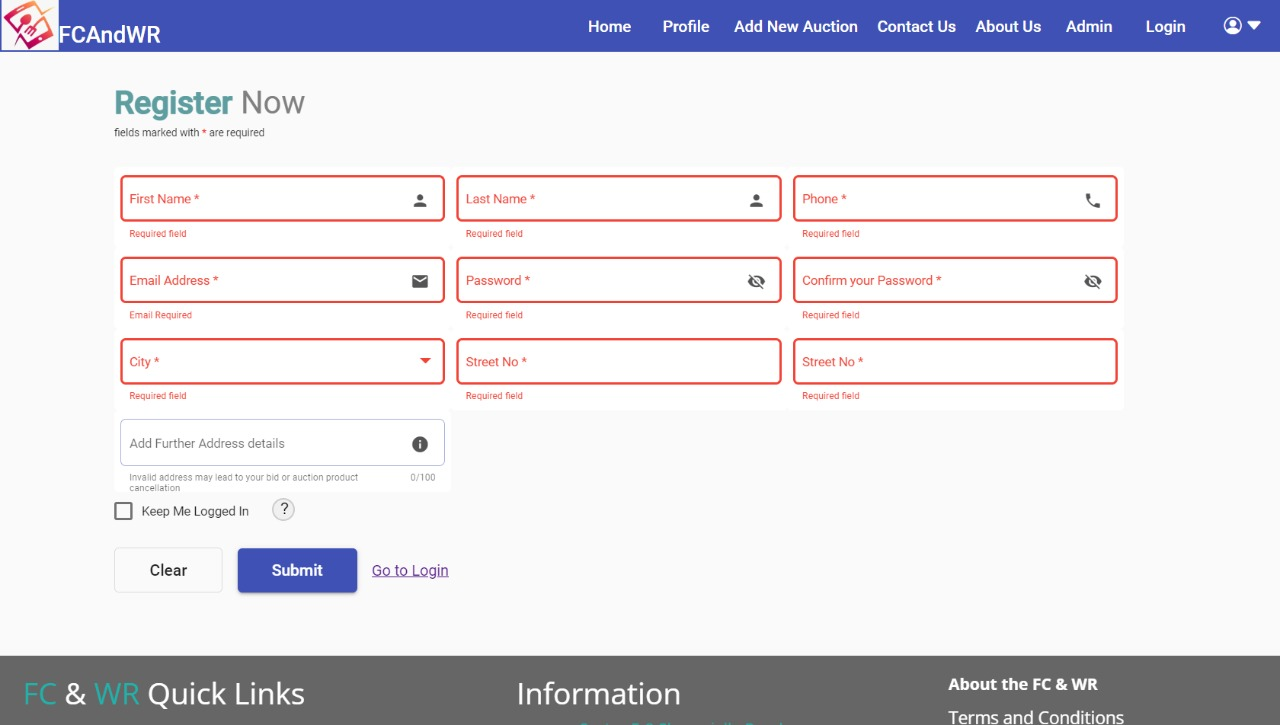
\includegraphics[width=15cm, height=15cm, keepaspectratio]{Responsive register page.jpeg}
    \caption{Responsive Registration}
    \label{rpr}
\end{figure}
\newpage
\subsection{Forgot Password}
If user forgets his password, then he will be sent a code to his registered email where he can recover his password. The forgot password page of our web application is shown in following Figure \ref{fp}.\\\\
\begin{figure}[!h]
    \centering
    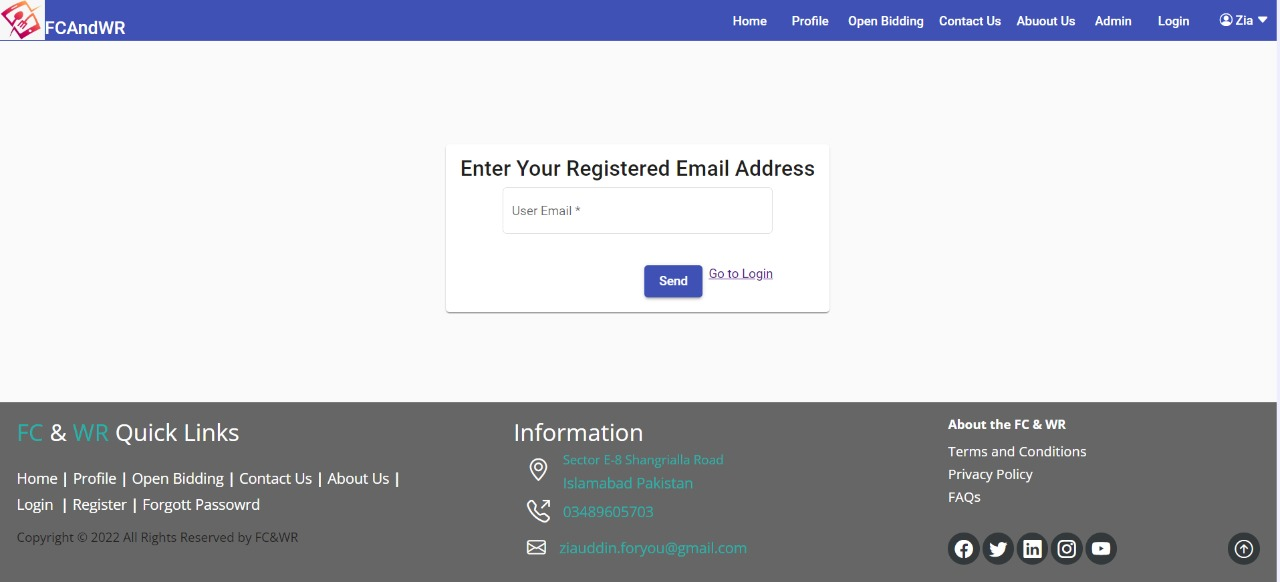
\includegraphics[width=15cm, height=15cm, keepaspectratio]{projectReportTemplate/figures/forgot.jpeg}
    \caption{Reset Password}
    \label{fp}
\end{figure}


\subsection{Profile Page}
This page shows the user purchase history and user sales history. when a user won a bid he will be able to see his won bid in his profile section. The profile page of our web application is shown in following Figure \ref{pp}.
\begin{figure}[!h]
    \centering
    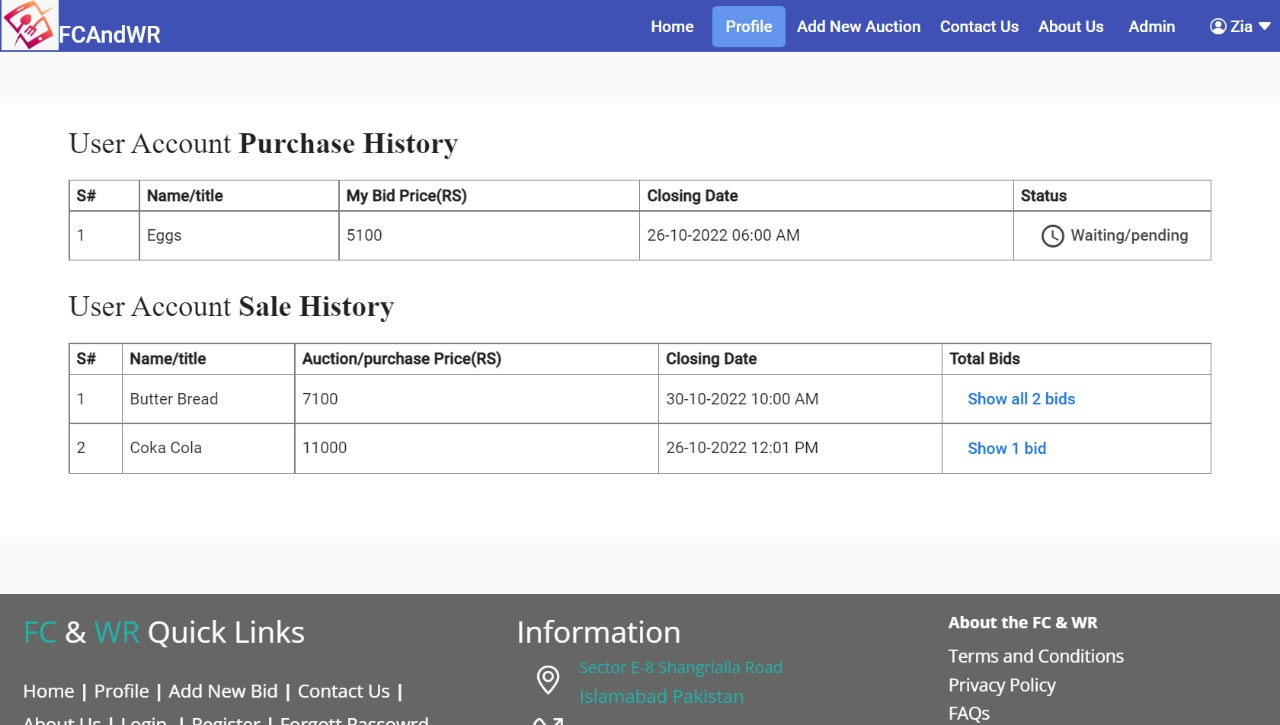
\includegraphics[width=15cm, height=15cm, keepaspectratio]{profile.jpeg}
    \caption{Profile Page}
    \label{pp}
\end{figure}

\subsection{Non-Login Profile Page}
This page shows the user purchase history and user sales history. when a user won a bid he will be able to see his won bid in his profile section. The non-login profile page of our web application is shown in following Figure \ref{nlpp}.
\begin{figure}[!h]
    \centering
    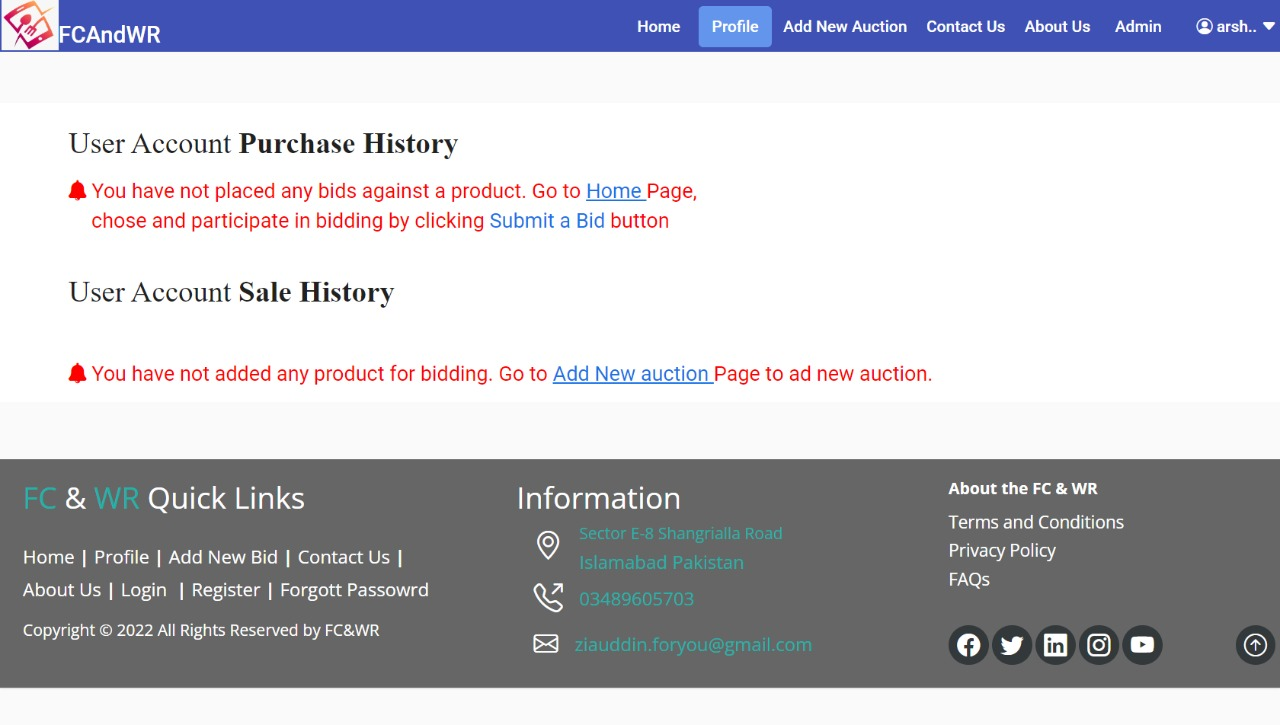
\includegraphics[width=15cm, height=15cm, keepaspectratio]{unlogin profile page.jpeg}
    \caption{Non-Login Profile Page}
    \label{nlpp}
\end{figure}
\newpage

\subsection{Checkout/Payment Page}
This page show the user purchase history and user sales history. when a user won a bid. He will be able to see his won bid in his profile section. The payment page of our web application is shown in following Figure \ref{co}.\\
\begin{figure}[!h]
    \centering
    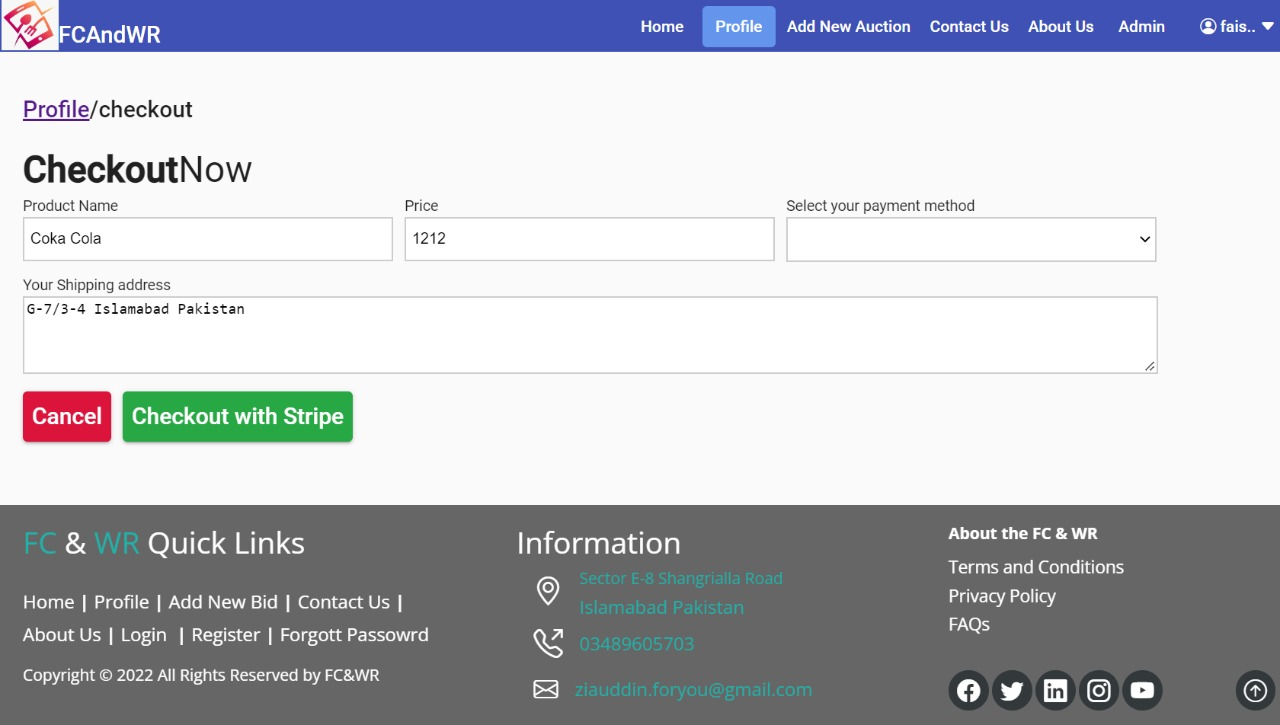
\includegraphics[width=15cm, height=15cm, keepaspectratio]{Checkout page.jpeg}
    \caption{Checkout/Payment Page}
    \label{co}
\end{figure}
\newpage
\subsection{Add New Auction Page}
In this page user will be able to add the information regarding the product he want to place on the bidding. He will enter product name, set it's price for auction and his address details. Finally he will add picture of the product and submit for new bid. The add new auction page of our web application is shown in following Figure \ref{ano}.\\\\
\begin{figure}[!h]
    \centering
    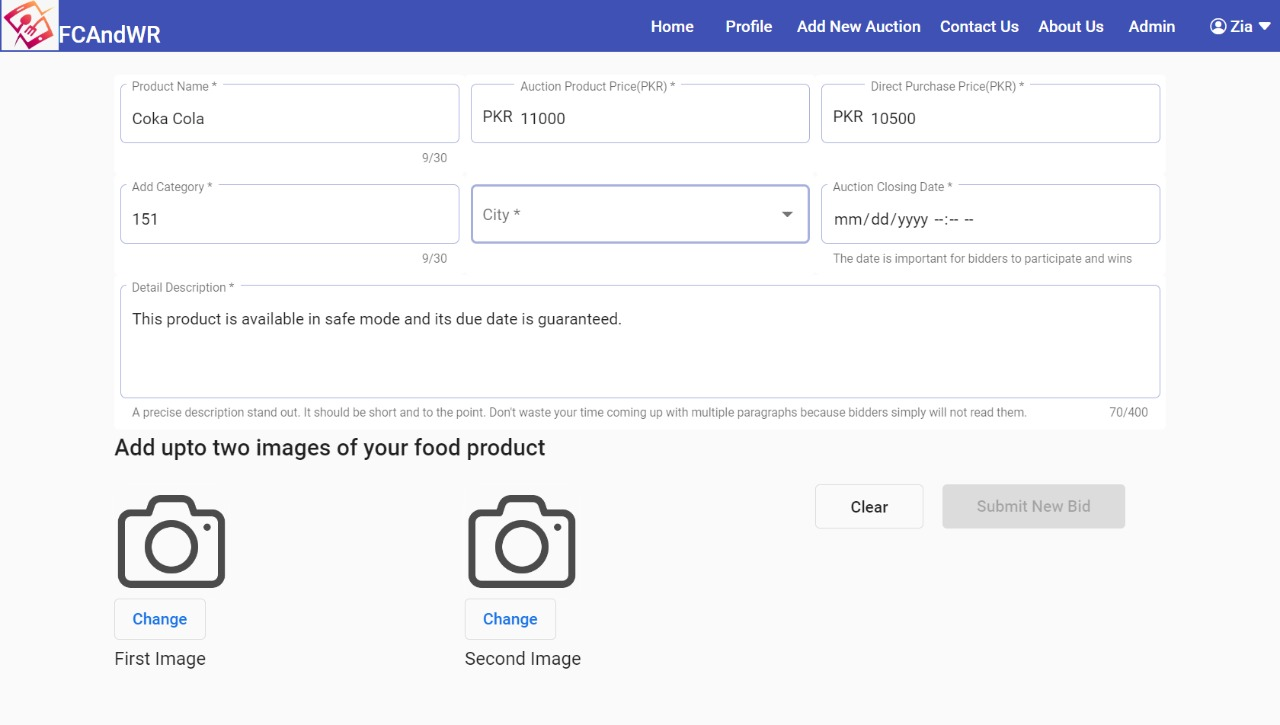
\includegraphics[width=15cm, height=15cm, keepaspectratio]{add new auction.jpeg}
    \caption{Add New Auction Page}
    \label{ano}
\end{figure}
\newpage
\subsection{Bid Detail Page}
In this page the buyer will be able to see the details of the product on auction and also he will be able to see time left for the bid. If he is interested then he will be able to place the bid. The bid detail page of our web application is shown in following Figure \ref{bdp}.\\\\
\begin{figure}[!h]
    \centering
    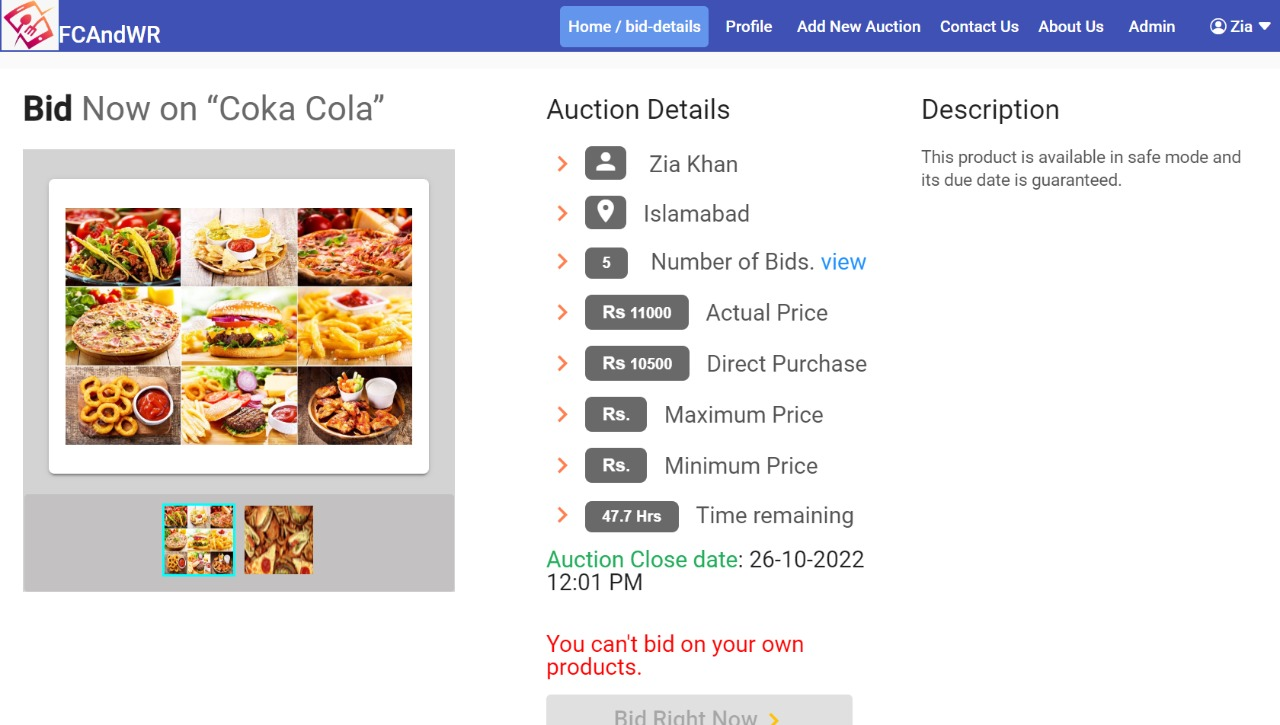
\includegraphics[width=15cm, height=15cm, keepaspectratio]{Bid details.jpeg}
    \caption{Bid Detail Page}
    \label{bdp}
\end{figure}
\newpage
\subsection{Bid Detail Update Page}
This is the extension of bid page when buyer select submit the bid then he enters the bid price that how much he is willing to pay for the product and also he can add a comment. The bid detail update page of our web application is shown in following Figure \ref{dbuo}.\\\\
\begin{figure}[!h]
    \centering
    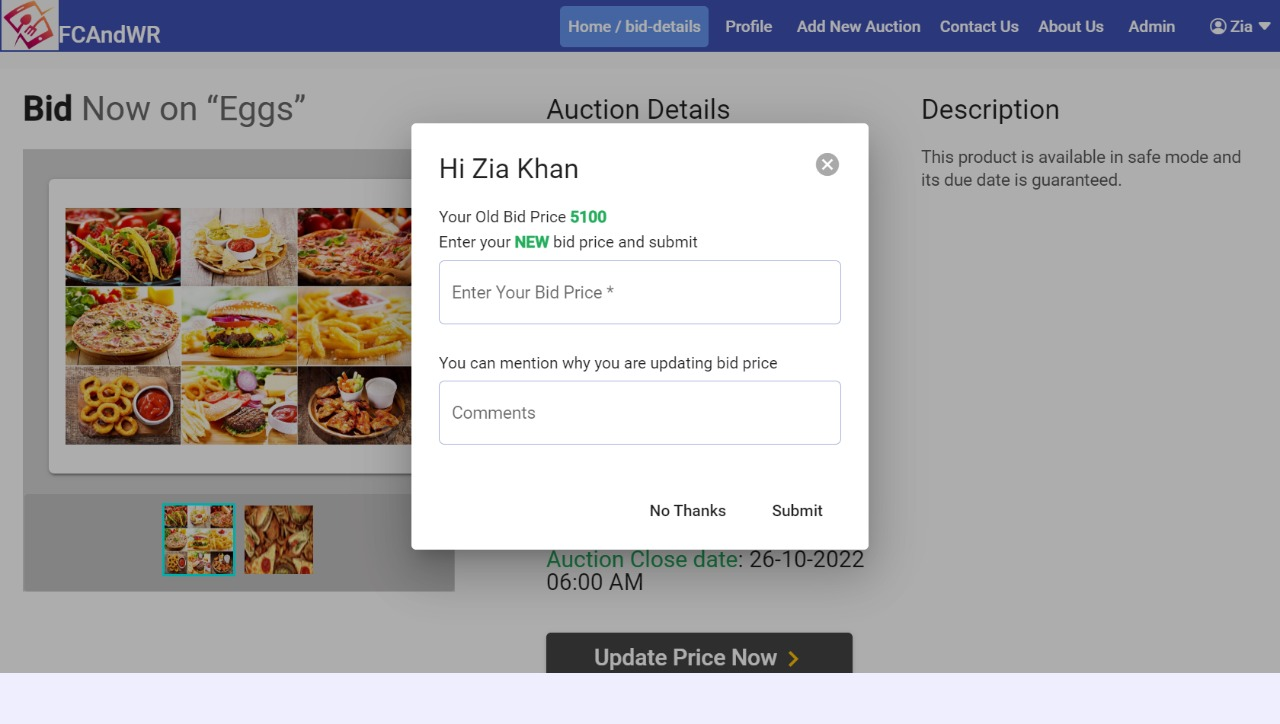
\includegraphics[width=15cm, height=15cm, keepaspectratio]{Bid details update.jpeg}
    \caption{Bid Detail Update Page}
    \label{dbuo}
\end{figure}
\newpage
\subsection{Contact Us Page}
If the user have an quarry then he can contact is through this page. The contact us page of our web application is shown in following Figure \ref{cu}.
\begin{figure}[!h]
    \centering
    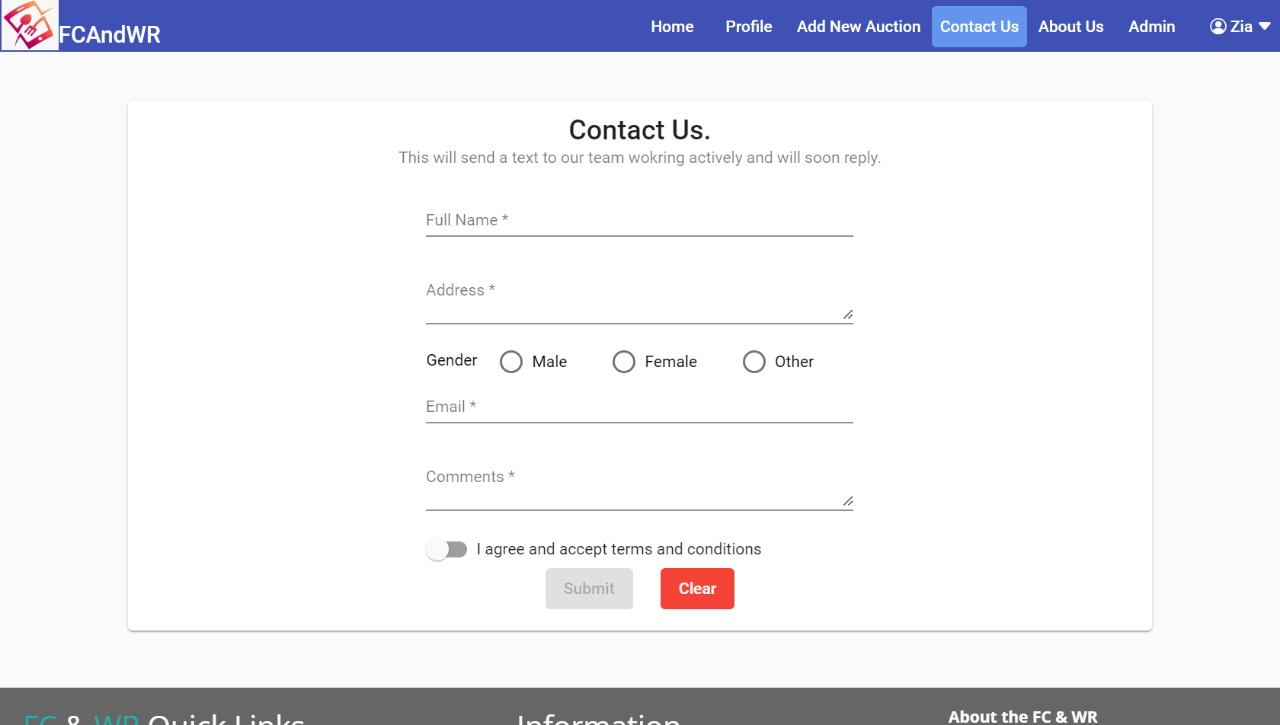
\includegraphics[width=15cm, height=15cm, keepaspectratio]{Contact us.jpeg}
    \caption{Contact Us Page}
    \label{cu}
\end{figure}
%\chapter{Chapter 8 title} \label{chap:concl}
%\version{v1.10.2015}
\section*{}
\lipsum

\section{Sec}
\lipsum
%%\printindex
%% comment next 2 commands if numbered appendixes not used
%%\appendix
%%\chapter{User Manual} \label{ap:Appendix1}

\section*{}
Appendices are provided to give supplementary information, which is included in the main text may serve as a distraction and cloud the central theme.

\begin{itemize}
	\item Appendices should be numbered using alphabets, e.g. Appendix A, Appendix B, etc.
	\item Tables and References appearing in appendices should be numbered and referred to at appropriate places just as in the case of chapters.
	\item Appendices shall carry the title of the work reported and the same title
shall be written in the contents page.
\end{itemize}
%\chapter{Appendix} \label{ap:appendix2}

\section*{}


%%----------------------------------------
%% Final materials
%%----------------------------------------

\begin{singlespace}
  %% Bibliography
  %% comment the next command if BibTeX file not used
  %% bibliography is in ``references.bib''
  \PrintBib{references}

  %% Index
  %% uncomment next command if index is required
  %% don't forget to run ``makeindex tese'' command
  \PrintIndex
\end{singlespace}

\end{document}